%% FEUP THESIS STYLE for LaTeX2e
%% how to use feupteses (English version)
%%
%% FEUP, JCL & JCF, 31 July 2012
%%
%% PLEASE send improvements to jlopes at fe.up.pt and to jcf at fe.up.pt
%%

%%========================================
%% Commands: pdflatex tese
%%           bibtex tese
%%           makeindex tese (only if creating an index)
%%           pdflatex tese
%% Alternative:
%%          latexmk -pdf tese.tex
%%========================================

\documentclass[11pt,a4paper,twoside,openright]{report}

%% For iso-8859-1 (latin1), comment next line and uncomment the second line
\usepackage[utf8]{inputenc}
%\usepackage[latin1]{inputenc}

%% English version

%% MIEIC options
\usepackage[mieic]{feupteses}
%\usepackage[mieic,juri]{feupteses}
%\usepackage[mieic,final]{feupteses}
%\usepackage[mieic,final,onpaper]{feupteses}

%% Additional options for feupteses.sty:
%% - onpaper: links are not shown (for paper versions)
%% - backrefs: include back references from bibliography to citation place

%% Uncomment the next lines if side by side graphics used
%\usepackage[lofdepth,lotdepth]{subfig}
%\usepackage{graphicx}
%\usepackage{float}

%% Include color package
\usepackage{color}
\definecolor{cloudwhite}{cmyk}{0,0,0,0.025}
\definecolor{bluekeywords}{rgb}{0.13,0.13,1}
\definecolor{greencomments}{rgb}{0,0.5,0}
\definecolor{redstrings}{rgb}{0.9,0,0}

%% Include source-code listings package
\usepackage{listings}
\lstset{ %
 language=[Sharp]C,                        % choose the language of the code
 basicstyle=\footnotesize\ttfamily,
 keywordstyle=\bfseries,
 numbers=left,                      % where to put the line-numbers
 numberstyle=\scriptsize\texttt,    % the size of the fonts that are used for the line-numbers
 stepnumber=1,                      % the step between two line-numbers. If it's 1 each line will be numbered
 numbersep=8pt,                     % how far the line-numbers are from the code
 frame=lr,
 float=htb,
 aboveskip=8mm,
 belowskip=4mm,
 rulecolor=\color{blue!80!black},
 backgroundcolor=\color{cloudwhite},
 showspaces=false,                  % show spaces adding particular underscores
 showstringspaces=false,            % underline spaces within strings
 showtabs=false,                    % show tabs within strings adding particular underscores
 tabsize=2,	                    % sets default tabsize to 2 spaces
 captionpos=b,                      % sets the caption-position to bottom
 breaklines=true,                   % sets automatic line breaking
 breakatwhitespace=false,           % sets if automatic breaks should only happen at whitespace
 escapeinside={\%*}{*)},            % if you want to add a comment within your code
 morekeywords={*,var,template,new}  % if you want to add more keywords to the set,
 commentstyle=\color{greencomments},
 keywordstyle=\color{bluekeywords}\bfseries,
 stringstyle=\color{redstrings}
}

%% Uncomment to create an index (at the end of the document)
%\makeindex

%% Path to the figures directory
%% TIP: use folder ``figures'' to keep all your figures
\graphicspath{{figures/}}

%%----------------------------------------
%% TIP: if you want to define more macros, use an external file to keep them
%some macro definitions

% format
\newcommand{\class}[1]{{\normalfont\slshape #1\/}}

% entities
\newcommand{\Feup}{Faculdade de Engenharia da Universidade do Porto}

\newcommand{\svg}{\class{SVG}}
\newcommand{\scada}{\class{SCADA}}
\newcommand{\scadadms}{\class{SCADA/DMS}}

%%----------------------------------------

%%========================================
%% Start of document
%%========================================
\begin{document}

%%----------------------------------------
%% Information about the work
%%----------------------------------------
\title{Exploring Visual Programming Concepts for Probabilistic Programming Languages}
\author{Gabriel Cardoso Candal}

%% Uncomment next line for date of submission
%\thesisdate{July 31, 2008}

%%Uncomment next line for copyright text if used
%\copyrightnotice{Name of the Author, 2008}

\supervisor{Supervisor}{Prof. Hugo Sereno Ferreira}

%% Uncomment next line if necessary
%\supervisor{Second Supervisor}{Name of the Supervisor}

%% Uncomment committee stuff in the final version if used
%\committeetext{Approved in oral examination by the committee:}
%\committeemember{Chair}{Doctor Name of the President}
%\committeemember{External Examiner}{Doctor Name of the Examiner}
%\committeemember{Supervisor}{Doctor Name of the Supervisor}
%\signature

%% Specify cover logo (in folder ``figures'')
\logo{uporto-feup.pdf}

%% Uncomment next line for additional text  below the author's name (front page)
%\additionalfronttext{Preparação da Dissertação}

%%----------------------------------------
%% Preliminary materials
%%----------------------------------------

% remove unnecssary \include{} commands
\begin{Prolog}
  \chapter*{Abstract}

Probabilistic programming is a way to create systems that help us make decisions
 in the face of uncertainty. Lots of everyday decisions involve judgment in
determining relevant factors that we do not directly observe. Historically, one
way to help make decisions under uncertainty has been to use a probabilistic
reasoning system.
Probabilistic reasoning combines our knowledge of a situation with the laws of
probability to determine those unobserved factors that are critical to the
decision. Typically, the way the several observations are combined is through
the usage of bayesian statistics, due to its anachronistic interpretation where
existing knowledge (priors) are combined with observations in order to gather
evidence towards competing hypothesis.

When compared to other machine learning methods (such as random forests, neural
networks or linear regression), which take homogeneous data as input (requiring
the user to separate their domain into different models), probabilistic
programming is used to leverage the data’s original structure. Plus, it
provides full probability distributions over both the predictions and
parameters of the model, whereas ML methods can only give the user some level
of confidence on the predictions.

Until recently, probabilistic reasoning systems have been limited in scope and
have been hard to apply to many real world situations. Models are communicated
using a mix of natural language, pseudo code, and mathematical formulae and
solved using special purpose, one-off inference methods. Rather than precise
specifications suitable for automatic inference, graphical models typically
serve as coarse, high-level descriptions, eliding critical aspects such as
fine-grained independence, abstraction and recursion.

Probabilistic programming is a new approach that makes probabilistic reasoning
systems easier to build and more widely applicable. A probabilistic programming
language (PPL) is a programming language designed to describe probabilistic
models, in a such a way we can say that the program itself is the model, and
then perform inference in those models. PPLs have seen recent interest from the
artificial intelligence, programming languages, cognitive science, and natural
languages communities. By empowering users with a common dialect in the form of
a programming language, rather than requiring each one of them to the non-trivial
and error-prone task of writing their own models and hand-tailored inference
algorithms for the problem at hand, it encourages exploration, since different
models require less time to setup and evaluate, and enables sharing knowledge
in the form of best practices, patterns and tools such as optimized compilers
or interpreters, debuggers, IDE’s, optimizers and profilers.

PPLs are closely related to graphical models and Bayesian networks but are
more expressive and flexible. One can quickly realize this by looking at the
re-usable components PPLs offer, being one of them the inference engine, which
can be plugged in into different models. For instances, it is easy to replace
the exact solution traditional Bayesian networks inference, which requires time
exponential in the number of variables to run, with approximation algorithms
such as the Markov Chain Monte Carlo (MCMC) or Variational Message Passing
(VMP), which make it possible to compute large hierarchical models by resorting
to sampling and approximation. PPLs often extend from a basic language (i.e.,
they are embedded in a host language like R, Java or Scala), although some PPLs
such as WinBUGS and Stan offer a self-contained language, with no obvious origin
in another language.

There have been successful applications of visual programming among several
domains, being it education (MIT’s Scratch and Microsoft’s VPL), general-purpose
programming (NoFlo), 3D modeling (Blender) and data science (RapidMiner and Wek
 Knowledge Flow). The latter, being popular products, have shown that there is
 added value in providing a graphical representation for working with data.
 However, as of today, no tool provides a graphical representation for a PPL.

DARPA, the main backer behind PPLs’ research, considers one of the main key
points of its Probabilistic Programming for Advancing Machine Learning program
to make models easier to write (reducing development time, encouraging
experimentation and reducing the level of expertise required to develop such
models). The use of visual programming is suitable for this kind of objectives,
so building upon the enormous flexibility of PPLs and the advantages of
probabilistic models, we want to take advantage of the graphical intuition given
by data visualization that data scientists are now accustomed to, and attempt
to provide model visualization by rethinking how to capture
the (usually textual) programmatic formalisms in a graphical manner.

We aim to overcome
the difficulties in learning a new language, either for inexperienced developers or seasoned
ones, such as learning yet another syntax or getting accustomed to the language’s idioms. It is
known that typical languages are difficult to learn and use \cite{Lewis1987} and that there are advantages in
providing a language with a visual interface \cite{dfbeg}.
The goal of this dissertation is thus to explore graphical representations of a
probabilistic programming language through the usage of visual programming.
The hypothesis under consideration is that graphical representations (not to be
confused with bayesian graphical model), are more intuitive and easy to learn
that full-blown PPLs.

We intend to validate such hypothesis by ensuring that classical problems solved
in the literature by PPLs are also supported by our graphical representation,
and then compare the two regarding understandability and error prevention.

During this dissertation we have developed a Visual Programming Environment (VPE),
a tool which allows the user to design its model graphically and then either
execute it or translate it into code. By doing so we have provided a tool which can be used to make usability research
on while also showing that it is possible
to represent a probabilistic program in a graphical manner by representing several
probabilistic programs with a variety of features using our tool.
 % the abstract
  % \chapter*{Acknowledgements}

Aliquam id dui. Nulla facilisi. Nullam ligula nunc, viverra a, iaculis
at, faucibus quis, sapien. Cum sociis natoque penatibus et magnis dis
parturient montes, nascetur ridiculus mus. Curabitur magna ligula,
ornare luctus, aliquam non, aliquet at, tortor. Donec iaculis nulla
sed eros. Sed felis. Nam lobortis libero. Pellentesque
odio. Suspendisse potenti. Morbi imperdiet rhoncus magna. Morbi
vestibulum interdum turpis. Pellentesque varius. Morbi nulla urna,
euismod in, molestie ac, placerat in, orci. 

Ut convallis. Suspendisse luctus pharetra sem. Sed sit amet mi in diam
luctus suscipit. Nulla facilisi. Integer commodo, turpis et semper
auctor, nisl ligula vestibulum erat, sed tempor lacus nibh at
turpis. Quisque vestibulum pulvinar justo. Class aptent taciti
sociosqu ad litora torquent per conubia nostra, per inceptos
himenaeos. Nam sed tellus vel tortor hendrerit pulvinar. Phasellus
eleifend, augue at mattis tincidunt, lorem lorem sodales arcu, id
volutpat risus est id neque. Phasellus egestas ante. Nam porttitor
justo sit amet urna. Suspendisse ligula nunc, mollis ac, elementum
non, venenatis ut, mauris. Mauris augue risus, tempus scelerisque,
rutrum quis, hendrerit at, nunc. Nulla posuere porta orci. Nulla dui. 

Fusce gravida placerat sem. Aenean ipsum diam, pharetra vitae, ornare
et, semper sit amet, nibh. Nam id tellus. Etiam ultrices. Praesent
gravida. Aliquam nec sapien. Morbi sagittis vulputate dolor. Donec
sapien lorem, laoreet egestas, pellentesque euismod, porta at,
sapien. Integer vitae lacus id dui convallis blandit. Mauris non
sem. Integer in velit eget lorem scelerisque vehicula. Etiam tincidunt
turpis ac nunc. Pellentesque a justo. Mauris faucibus quam id
eros. Cras pharetra. Fusce rutrum vulputate lorem. Cras pretium magna
in nisl. Integer ornare dui non pede. 

\vspace{10mm}
\flushleft{The Name of the Author}
  % the acknowledgments
  \cleardoublepage
\thispagestyle{plain}

\vspace*{8cm}

\begin{flushright}
   \textsl{``You should be glad that bridge fell down. \\
           I was planning to build thirteen more to that same design''} \\
\vspace*{1.5cm}
           Isambard Kingdom Brunel
\end{flushright}
       % initial quotation if desired
  \cleardoublepage
  \pdfbookmark[0]{Table of Contents}{contents}
  \tableofcontents
  \cleardoublepage
  \pdfbookmark[0]{List of Figures}{figures}
  \listoffigures
  \cleardoublepage
  \pdfbookmark[0]{List of Tables}{tables}
  \listoftables
  \chapter*{Abbreviations}
\chaptermark{ABBREVIATIONS}

\begin{flushleft}
\begin{tabular}{l p{0.8\linewidth}}
ADT      & Abstract Data Type\\
API      & Application Programming Interface\\
CLI      & Common Language Infrastructure\\
CLR      & Common Language Runtime\\
DARPA    & Defense Advanced Research Projects Agency\\
DOM      & Document Object Model\\
DPL      & Dataflow Programming Language\\
EBNF     & Extended Backus–Naur Form\\
ML       & Machine Learning\\
IDE      & Integrated Development Environment\\
JIT      & Just in Time\\
JVM      & Java Virtual Machine\\
PP       & Probabilistic Programming\\
PPAML    & Probabilistic Programming for Advancing Machine Learning\\
PPL      & Probabilistic Programming Language\\
PR       & Probabilistic Reasoning\\
PVL      & Purely Visual Language\\
VDP      & Visual Dataflow Programming\\
VMP      & Variational Message Passing\\
VP       & Visual Programming\\
VPE      & Visual Programming Environment\\
VPL      & Visual Programming Language\\
XML      & eXtensible Markup Language
\end{tabular}
\end{flushleft}
  % the list of abbreviations used
\end{Prolog}

%%----------------------------------------
%% Body
%%----------------------------------------
\StartBody

%% TIP: use a separate file for each chapter
\chapter{Introduction} \label{chap:intro}

\section*{}

This first chapter aims to provide the reader with an overview of this
dissertation. It starts by introducing the context this work is inserted in,
identifying the problem which we aim to solve, how we plan on solving it, and
the expected outcome. Lastly, it gives a bird's eye view of this report's
structure.

\section{Context} \label{sec:context}

There is, among several domains with interesting and relevant problems to solve
(computer vision \cite{Kulkarni2015}, cryptography, biology, fraud detection,
recommender systems \cite{intml}, …), the recurring necessity to be able to
make decisions in the face of uncertainty using machine learning (ML) methods.

Successful ML applications include Google's personalized advertising and
context-driven information retrieval, Facebook's studies of how information
spreads across a network or UC Berkeley's AMPLab contributions towards Amazon
Web Service and SAP's products \cite{Broder:2015:BDN:2684822.2697027}.

Typically, there are two alternatives for solving this class of problems: either use an
existing machine learning model (such as KNN, neural networks or similar) \cite{mlnot} and
try to fit your data into the model, or build a probabilistic model for your
own particular problem so you can better leverage domain knowledge \cite{SciPy}.

In the second alternativa one common way to approach0 it is by using bayesian reasoning,
where you model unknown causes with random variables, feed the model the data you
have gathered and then perform inference to query for the
desired, and previously unknown, variables \cite{thbay}. The problem in choosing
this method is this last step, since it is non-trivial
to write an inference method \cite{Duvenaud}.

The solution to this has been building generic inference engines for graphical
models, so that modeling and inference can be treated as separate concerns and
people can focus on the modeling \cite{Jordan1996}. However, not all models can be represented as
graphical models, and that’s why we now have Probabilistic Programming Languages
(PPLs). Probabilistic Programs let you write your model as a program and have
off-the-shelf inference \cite{Prekopa2003}.

\section{Problem} \label{sec:proj}

In spite of these examples of applications in the industry, ML has been
identified by Gartner, in its Hype Cycle annual review,
to be in the "Peak of Inflated Expectations" stage, still far
from the "Plateau of Producitvity" \cite{gartner}.

It has also been said that ML's applications are rarely seen
outside the academia, with Wagstaff claiming that there is a "frequent lack of
connection between machine learning research and the larger world of scientific
inquiry and humanity" \cite{Wagstaff2012}.

Arguably the scenario is even worse for PPLs, having even lesser adoption
among tech companies. One factor which may be contributing to this lack of
usage, despite PP's power and flexibility, is the difficulty for data scientists
to adapt to textual interface these languages provide, which lack the graphical
intuiton provided by other tools they are accustomed to. In a poll made to about 2800
data scientists (see Figure \ref{fig:poll}), half of the top 10 tools are
graphically-interactable.

\begin{figure}[t]
  \begin{center}
    \leavevmode
    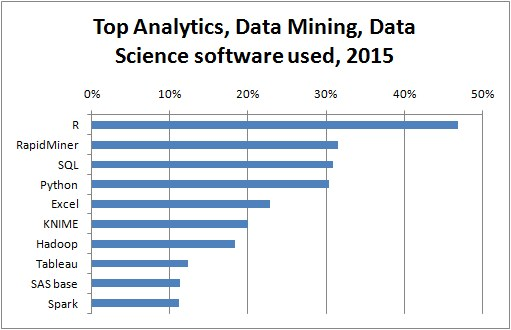
\includegraphics[width=0.86\textwidth]{poll}
    \caption{Top 10 Analytics Tools \cite{kdn}}
    \label{fig:poll}
  \end{center}
\end{figure}

\section{Motivation and Goals} \label{sec:goals}

The Defense Advanced Research Projects Agency (DARPA), one of the funders behind
PPLs' research, has recognized some of the problems
identified by Wagstaff and started a program called Probabilistic Programming
for Advancing Machine Learning (PPAML) to address the shortcomings of
current ML methods \cite{darpa}. It identifies five strategic goals:

\begin{itemize}
  \item Shorten machine learning model code to make models faster to write and
  easier to understand
  \item Reduce development time and cost to encourage experimentation
  \item Facilitate the construction of more sophisticated models that
  incorporate rich domain knowledge and separate queries from underlying code
  \item Reduce the level of expertise necessary to build machine learning
  applications
  \item Support the construction of integrated models across a wide variety of
  domains and tool types
\end{itemize}

The purpose of this work is to try addressing the first four. In order to do so we
aim to overcome the difficulties in learning a new language, either for
unexperienced developers or seasoned ones, such as learning yet another syntax
or getting accostumed to the language's idioms. It is known that typical
languages are difficult to learn and use \cite{empstud} and that there are
advantages in providing a language with a visual interface \cite{dfbeg}. Also,
studies have shown that programmers and data scientists alike resort to mental
imagery when solving problems \cite{Dastani2002}\cite{Petre1999}, so by
providing such an interface we can approximate how people think and how they
use the language to solve the problem at hand.

So, the goal of this dissertation will be to develop a Visual Programming
Language (VPL) with probabilitics programming capabilities. The targeted
audience are programmers and data scientists with background knowledge in
statistics who aren't still comfortable
with full blown PPLs, but wish to educate themselves in the topic so they can
eventually leverage the power of this novel machine learning approach.

The way to do so would be developing a graphical node-based editor, similar to
RapidMiner or Blender Composite Nodes, but that runs in the browser. The given
editor would have the capability to compile its graph to the textual
representation in the target PPL so that the user can run what it has designed,
either as a standalone script or even by integrating it with his existing
projects.

The hypothesis under consideration is this graphical representation
is more intuitive and easy to learn that a full-blown PPL.
We intend to validate such hypothesis by ensuring that classical problems solved
in the literature by PPLs are also supported by our graphical representation,
and then measure how quickly a group of people trained in statistics would
produce a viable model in both alternatives.

\section{Outline} \label{sec:struct}

Para além da introdução, esta dissertação contém mais x capítulos.
No capítulo~\ref{chap:sota}, é descrito o estado da arte e são
apresentados trabalhos relacionados.
%\todoline{Complete the document structure.}
No capítulo~\ref{chap:chap3}, ipsum dolor sit amet, consectetuer
adipiscing elit.
No capítulo~\ref{chap:chap4} praesent sit amet sem.
No capítulo~\ref{chap:concl}  posuere, ante non tristique
consectetuer, dui elit scelerisque augue, eu vehicula nibh nisi ac
est.

\chapter{Background \& State of the Art} \label{chap:sota}

\section*{}

This chapter has two purposes: describing the foundations on which this work
is built on, namely Machine Learning (ML), Probabilistic Reasoning (PR),
Probabilistic Programming (PP) and
Visual Programming(VP) while enumerating different tools which are based
on one or several of these concepts.

\section{Machine learning}

Machine learning (ML) is a field which can be seen as a subfield of artificial
intelligence that incorporates mathematics and statistics and is concerned
with conceiving algorithms that learn autonomously, that is, without human
intervention \cite{mlbrit}\cite{mlnot}.
It has the potential to impact a wide spectrum of
different areas such as biology, medicine, finance, astronomy
\cite{Amatriain:2013:BDU:2541176.2514691}, computer vision, sales forecast,
robotics \cite{intml}, product recommendations, fraud detection or
internet ads bidding \cite{SciPy}.

Learning from data is commercially and scientifically important. ML consists of
methods that automatically extract interesting knowledge in databases of sometimes chaotic and
redundant information. ML is a data-based knowledge-discovering process that
has the potential not only to analyze events in retrospect but also to predict
future events or important alterations \cite{mapt}.

\section{Probabilistic Reasoning}

Probabilistic reasoning (PR) is the formation of probability judgments and of
informed yet subjective beliefs about the likelihoods of outcomes and the frequencies of
events \cite{Lassiter2012}, it is a way to combine our knowledge of a situation
with the laws of probability. There are subjective beliefs because in non-trivial
decision-making there is a combination of unobserved factors that are critical to the decision
and several sources of uncertainty \cite{reas}, such as:

\begin{itemize}
  \item Uncertain inputs, due to missing or noisy data.
  \item Uncertain knowledge, where multiple causes lead to multiple effects,
  or there is an incomplete knowledge of conditions, effects and causality of the
  domain or simply because the effects are inherently stochastic.
\end{itemize}

So, probabilistic reasoning only gives probabilistic results and it is one way to
overcome cognitive bias and be able to make rational decisions \cite{Sedlmeier2001}.

A trial has been made \cite{christensen1982experience}
where physicians were asked to estimate the probability that a
woman with a positive mammogram actually has breast cancer, given a base rate of
1\% for breast cancer, a hit rate of about 80\%, and a false-alarm rate of about
10\%. It reported that 95 of 100 physicians estimated the probability that she
actually has breast cancer to be between 70\% and 80\%, whereas Bayes's rule
gives a value of about 7.5\%. Such systematic deviations from Bayesian reasoning
have been called "cognitive illusions". We will describe both Bayes' rule
and Bayesian reasoning in the next section.

\subsection{Bayesian Reasoning}
\label{sec:bayes}

One way to approach PR is by using bayesian reasoning, which is inspired in the
Bayes Theorem (or Rule, or Law). An equivalent formula to the theorem, in its
simplest form (applied to a single event) is:

$$ P(A \mid B) = \frac{P(A \land B)}{P(B)} $$

Where P(A|B) defines the probability of event A given that B occurred.
The theorem defines how hidden causes (A) relate to observed events (B), given
a causality model (P(A, B) or P(B|A)*P(A)) and our knowledge of the probability of the
occurrence of events (P(B)). The inverse is also true, as we will see further
ahead in this section.
As an example, P(penalty | goal) defines the probability that a penalty kick was
scored, knowing that there was a goal.

There are at least two interpretations to the theorem and regarding how one may think
about its results \cite{Fienberg2006}:

\begin{itemize}
  \item Frequentist interpretation: probabilities are defined by the relative
frequency of events, given a natural sampling. Meaning, the probability of
obtaining 'Heads' when rolling a dice is equal to the number of 'Heads' obtained
after rolling the dice a sufficient number of times relative to the total number
of times the dice has been rolled.
  \item Epistemological interpretation: probabilities represent a measure of
belief. It can either be a result logical combination of probabilities through
the usage of axioms (it's closely related to Aristotelian logic)
or it can also reflect a personal belief (which is called a subjective view).
\end{itemize}

\subsubsection{An example}

One example of the application of this theorem is \cite{reas}: you know your home's alarm
is ringing, but you don't know whether that was caused by a burglar or
something else (maybe a bird triggered it, or there was a malfunction in the
alarm system). How confident are you that you're being robbed? Consider that
the alarm company, based on quality trials, defined in the confusion
matrix for P(alarm, burglary) (Table \ref{tab:bayes}).

\begin{table}[t]
  \centering
  \caption{Alarm system confusion matrix}
\begin{tabular}{| l | l | l |}
	\hline
  & alarm & \neg alarm \\ \hline
 burglary & 0.09 & 0.01 \\ \hline
 \neg burglary & 0.1 & 0.8 \\ \hline
\end{tabular}
  \label{tab:bayes}
\end{table}

You can interpret each table's cell as P(A, B). For instances, the top left
cell is the probability that the alarm rings and there is a burglar, while the
bottom left cell is the probability that the alarm rang but there was no burglar
(a false positive).

If we substitute the values of Bayes' rule described above, we get:

$$ P(burglar \mid alarm) = \frac{P(burglar, alarm)}{P(alarm)} $$

Where results is 0.09 / 0.19 = 0.47. So, even if the alarm is ringing, there is
just a 47\% probability that the house is actually being robbed.

The previous example illustrates the simplest case of applied BR, but it is
also possible to combine several variables.
One way to represent this kind of scenario is by expressing the variables in a directed acyclic
graph, where the relation "Parent" stands for "May cause" and you can specify
the conditional probabilities of a child given a parent's result. This graphical
model is called a Bayesian Network.

\subsubsection{Bayesian Networks}

We can extend our alarm example further, by considering not only a burglar
can trigger the alarm, but an earthquake also can (while there can still be
false positives). Also, consider that we have 2 neighbors (Mary and John) who
may call us whether the alarm is ringing or not. This problem is represented in
figure \ref{fig:beliefnet}.

\begin{figure}[t]
  \begin{center}
    \leavevmode
    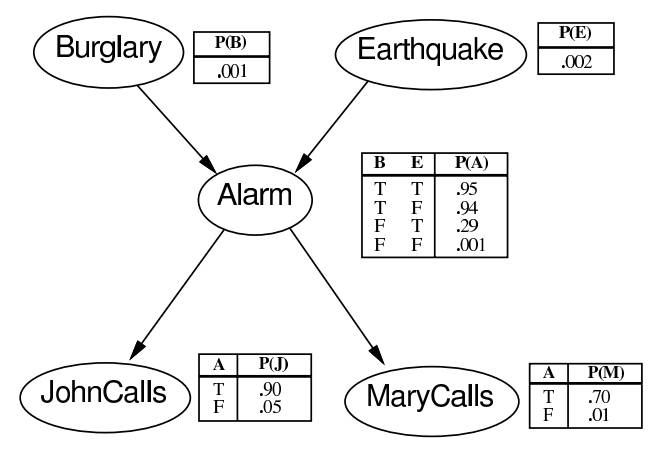
\includegraphics[width=0.86\textwidth]{beliefnet}
    \caption{Belief network for the alarm problem \cite{belfn}}
    \label{fig:beliefnet}
  \end{center}
\end{figure}

Some interesting question we can ask, given this scenario are:

\begin{itemize}
  \item If John calls saying the alarm is ringing but Mary doesn't, what are the
odds it really is ringing?
  \item If the alarm is ringing, was there an earthquake?
  \item What are the chances that both my neighbors call, the alarm is ringing,
but there is neither a burglary nor an earthquake?
\end{itemize}

This last example, for instances, would be calculated as: P(J, M, A, \neg B, \neg E)
= P(J|A) * P(M|A) * P(A|\neg B, \neg E) * P(\neg B) * P(\neg E) =
0.9 * 0.7 * 0.001 * 0.999 * 0.998 = 0.00062.

Notice how counter-intuitive this
example is: the probability of there being an earthquake is about 32 times larger
than there being an earthquake, the alarm ringing and the neighbors calling us,
even if the conditional probabilities are reasonably high (0.95, 0.9 and 0.7).
This is the result of the calculation of the joint probability being an highly
combinatorial problem, which is yet another argument in favor of using PR
rather than subjective heuristics.

\subsubsection{Bayes' and data streams}

In practical ML applications, it is often the case that there is an
incoming stream of new data, rather than one-time batch calculations.
BR can accommodate this way of thinking, which A. Downey called diachronic
interpretation \cite{thbay}, where diachronic means that something is happening
over time (in this case the probability of the hypotheses, as new data arrives).
In order to make sense of this definition, we may rewrite Bayes' rule as:

$$ P(H \mid D) = \frac{P(D \mid H) \, P(H)}{P(D)} $$

Where:

\begin{itemize}
  \item H: hypothesis
  \item D: data
  \item p(H): probability of the hypothesis before the new data is taken into
account. Also called \textbf{prior}. It can either be calculated using background
information or subjectively defined using domain knowledge. Loses significance
as new data is added, so its choice is not determinant to the model's performance
in the long run.
  \item p(H|D): what we want to calculate, the probability of the hypothesis
after considering the new date. It is called \textbf{posterior}.
  \item p(D|H): probability of the data if the hypothesis was true, called
the \textbf{likelihood}.
  \item p(D): probability of the data under any hypothesis, called the
\textbf{normalizing constant}.
\end{itemize}

Under this interpretation, you may continuously feed data into the model and see
the probabilities getting updated. We will see more practical examples of this
in section \ref{sec:pp}.

\subsubsection{Beyond Bayesian Graphical Model}

At first glance, someone who is learning for the first time about PR applied
to ML, may think that graphical models such as the one presented in Figure
\ref{fig:beliefnet} are the best there can be done in terms of using a graphical
interface for solving this kind of problems and that the only thing is missing
is an automated way to make the calculations.

While it is true we have still never mentioned techniques or tools that
automatically do inference over a Bayesian Network, there are several tools
with that capability (including an R package \cite{Hojsgaard2013} or
standalone tools \cite{msbn}).

However, not all PR can be done via Bayesian Networks and not all graphical models
are enough for complete PR \cite{intpp}. PP are the largest class of models available, and there are
also more algorithms for inference than just the calculation of joint
probabilities (like we did in the alarm example), as we will discuss in Section
\ref{sec:pp}.

Bayesian Networks are not the only kind of graphical model. Another one would be
Markov Chains, which is yet another example of a model which is not able to
represent all PR problems. This is clear when we realize that, while PPLs
support numerous distributions (such as Normal, Laplace,
Gamma, Half-Cauchy or \textit{t}), all Bayesian Networks and Markov Chain
can be represented in a PPL by just using Bernoulli distributions \cite{PPm}.
We can see an example of such a translation in Figure \ref{fig:mppl}.

\begin{figure}[t]
  \begin{center}
    \leavevmode
    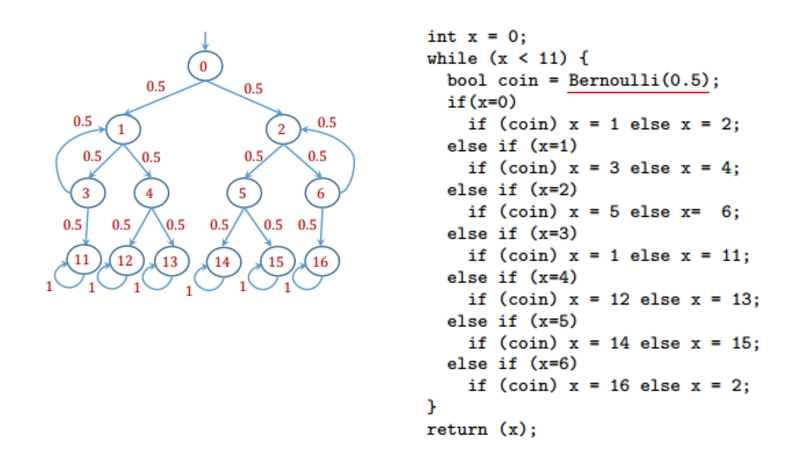
\includegraphics[width=0.86\textwidth]{markppl}
    \caption{Translation of Discrete Time Markov Chain to a PPL \cite{PPm}}
    \label{fig:mppl}
  \end{center}
\end{figure}

% <---- TODO rever com base em prob inference for graphical models

\subsection{Probabilistic Programming Languages}
\label{sec:pp}

\subsubsection{The Probabilistic Program-Model duality}

A probabilistic program (PP) is an ordinary program (that can be written in
mainstream languages such as C, Java or Haskell) whose purpose is to specify
a probability distribution of its variables. This is done by sampling over
several executions of the program. The only needed construct the language
has to support, in order to be able to write a PP, is having a random number
generator \cite{intpp}. This whole concept couldn't be better explained than in this text by Freer and
Roy, regarding Church (a PPL, which we describe in Section \ref{sec:church})
but common to any PP:

\begin{quote}
  ``If we view the semantics of the underlying deterministic language as a map
  from programs to executions of the program, the semantics of a PPL built on it
   will be a map from programs to distributions over executions. When the
   program halts with probability one, this induces a proper distribution over
   return values. Indeed, any computable distribution can be represented as the
   distribution induced by a Church program in this way''~\cite{Freer2012}
\end{quote}

One way to think about this notion is by considering that the program itself
is the model. An example of the relation between a model (expressed in a PPL)
and the implied distribution over its variables (obtained using an inference
method) can be seen in Figure \ref{fig:distribution}, where a variable \textit{flip}
is set to be a Bernoulli distribution and \textit{x} is defined in terms of
\textit{flip}. We can then see how the graphic of the inferred distributions
of \textit{flip's} and \textit{x's} values looks like and confirm what was to
be expected: for \textit{flip's} values lower than 0.5 we see \textit{x} follows
a normal distribution, whereas for values greater than 0.5 it follows a gamma
distribution instead.
 The goal of PP (via PPL) is to enable PR and ML to be accessible to
most programmers and data scientists who have enough domain and programming
knowledge but not enough expertise in probability theory or machine learning.

\begin{figure}[t]
  \begin{center}
    \leavevmode
    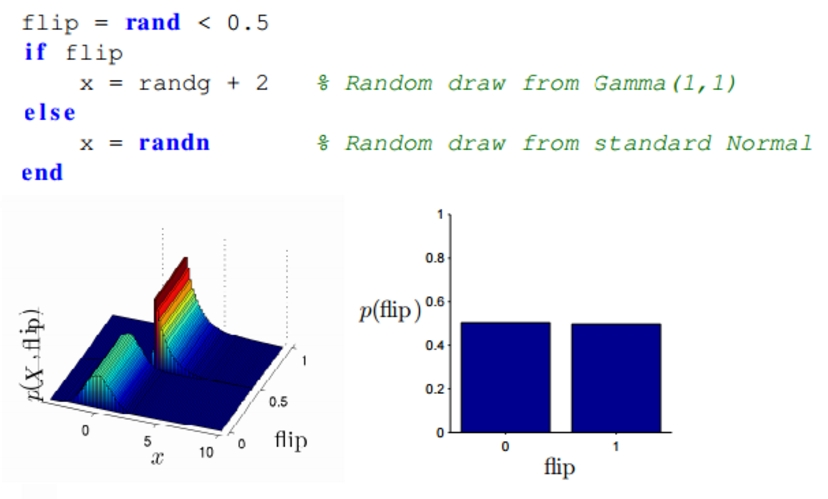
\includegraphics[width=0.86\textwidth]{distribution}
    \caption{Implied distributions over variables \cite{intpp}}
    \label{fig:distribution}
  \end{center}
\end{figure}

\subsubsection{PPLs vs regular PLs}

What is then, a Probabilistic Programming Language (PPL)? First of all, it can
be a standalone language or an extension to a general purpose programming language.
We'll be analyzing examples of languages from either these categories in Section
\ref{sec:art}, but many more exist, such as Figaro \cite{figaro} (hosted in Scala),
webppl \cite{dippl} (embedded in javascript) or Dimple
\cite{DBLP:journals/corr/abs-1212-2991} (which has both a Java and a MATLAB API).
The key difference between these languages and a PPL is the latter has
the added capability of performing conditioning and inference \cite{Andrieu2003}.

Conditioning is the ability to introduce observations about the real world in
the program. That way, you update the prior probability based
on those observations. Consider the example in Figure \ref{fig:truskill} (which
is a simplified version of how Microsoft applies PP in its Xbox matchmaking
algorithm \cite{minka2012infer}) where the prior is a normal distribution with
equal parameters for all players (shown by the graphic in the top). Then, it
defines how the performance of the player is based on his skill (which at the initial
point in time, is equal to every one of them) and proceeds to make several
observations regarding games between them. Finally, it shows the inferred
probability distribution of the posterior on the bottom graphic.

\begin{figure}[t]
  \begin{center}
    \leavevmode
    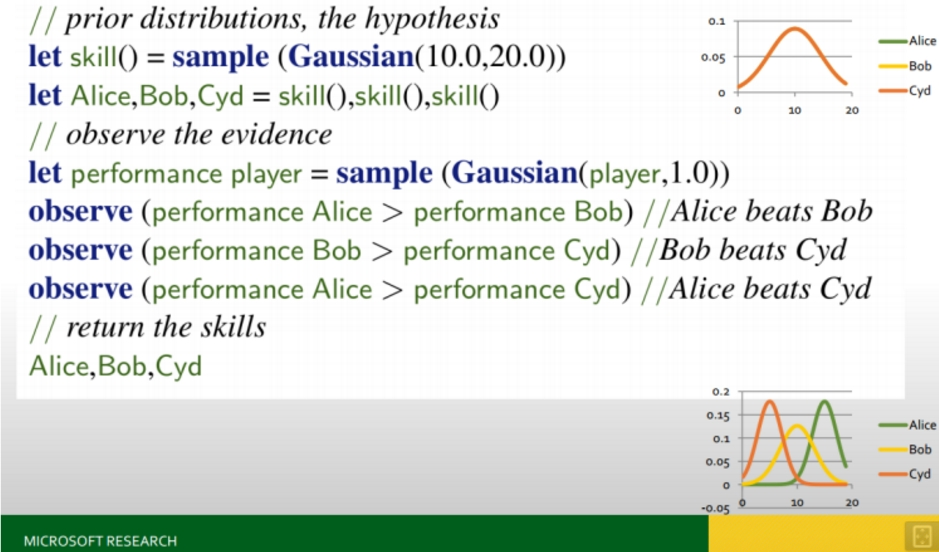
\includegraphics[width=0.86\textwidth]{trueskill}
    \caption{Microsoft Xbox Live True Skill \cite{minka2012infer}}
    \label{fig:truskill}
  \end{center}
\end{figure}

\subsubsection{Inference}

We said that a PPL empowers the user to formalize a model and then query for the
probability distribution of its variables, which is automatically done via
inference. While general-purpose language require you to write one-time
inference methods that tightly coupled to the PP you are inferring on, PPLs
ship with an inference engine suited to most PP programs you can write
\cite{Freer2010}.

An inference engine of a PPL acts similarly to a compiler in a traditional
language: rather than requiring each user to engineer its own, which requires
significant expertise and is a non-trivial and error-prone endeavor, every PPL
has one incorporated.

Having the inference engine work as a separate component, rather than being
tightly coupled to each model, opens up a myriad of new
possibilities mainly in the form of knowledge and tool sharing, as we have
seen in the past in the compiler space. Examples of this would be new
compiler and interpreter techniques (such as working towards scalability or
parallelization), optimizers, profilers or debuggers.

Another great advantage of having a modular inference engine is that we can
try different inference algorithms and pick the one that best fits the problem
at hand. When analyzing which algorithm is more suitable for a certain use case, there are certain
characteristics worth noting \cite{Minka1999}:

\begin{itemize}
  \item Determinism - in equal initial conditions, an algorithm always yields
the same result.
  \item Exact result or approximation.
  \item Guaranteed convergence - an algorithm may or not be guaranteed to reach
a result at some point in time. If not, it's possible that it will run forever.
  \item Efficiency - related to how fast can it reach a result.
\end{itemize}

Microsoft's Infer.NET provides three inference algorithms \cite{msalg}:

\begin{itemize}
  \item Expectation Propagation - deterministic, provides exact solutions only
in some cases, is not guaranteed to converge and is labeled as "reasonably
efficient".
  \item Variational Message Passing - also deterministic, but always gives
approximates results and is guaranteed to converge. It's considered to be the
most efficient of the three for most cases.
  \item Gibbs sampling - non-deterministic, may be able to reach exact result
if given enough time to run, has guaranteed convergence and is regarded as
not-so-efficient as the other two.
\end{itemize}

We can divide the three algorithms into two categories: variational bayesian
methods \cite{Winn2005}\cite{Minka1999} and sampling methods (in the case of Gibbs
sampling, it's based on Markov chain Monte Carlo) \cite{Andrieu2003}. The main
difference, as far as the end-user is concerned, is that variational methods
provide faster results but are subject to bias, whereas sampling methods have
the potential to produce more accurate results (the downside being it's slower
and its convergence is hard to diagnose) \cite{Shen2010}.

Please notice that none of these algorithms provides the same kind of exact
solution as the calculation of the joint probabilities we did in Section
\ref{sec:bayes}. The reason for that is that calculating an exact solution
takes time exponential in the number of variables to run, even if we have smarter
algorithms than the naive calculations we did \cite{Zhang1994}.

\subsubsection{Openbox models}

When compared to traditional machine learning methods (such as random forests, neural
networks or linear regression), which take homogeneous data as input (requiring
the user to separate their domain into different models), probabilistic
programming is used to leverage the data’s original structure. This is done by
empowering the user to write his own models while taking advantage of a re-usable
inference engine. Olivier Grisel called this combination "Openbox models,
blackbox inference engine"\cite{SciPy}.

Rather than using most of his
time performing feature engineering (that is, trying to fit the problem and the
data into an existing model), the user will have the tool necessary to design
the model that best fits the domain he is working on.
Plus, it provides full probability distributions over both the predictions and parameters of the
model, whereas ML methods can mostly only give the user a certain degree of confidence
on the predictions.

\subsection{Conclusion}

Summarizing, PPLs are a step forward in using PR to solve ML problems since
it helps overcome the difficulties in using PR in real world problems. This is
done by adding automated general inference on top of a precise specification
(the program), where in the past models were communicated
using a mix of natural language, pseudo code, and mathematical formulae and solved
using special purpose, one-off inference methods.

This encourages exploration, since
different models require less time to setup and evaluate, and enables sharing
knowledge in the form of best practices and design and development patterns.

However, using a full fledged programming language might still be an entry
barrier. We want to help statisticians and data scientists alike to learn
faster and be more productive using a PPL in a way similar to the tools they
are accustomed to. In order to do so, we'll be combining a PPL with Visual
Programming (Section \ref{sec:vp}).

\section{Visual Programming}
\label{sec:vp}

Visual Programming (VP) can be defined as "any system that allows the user to specify a program in a
two-(or more)-dimensional fashion." \cite{Myers1986}.
In a textual programming language, even though there are two dimensions (one
being the text itself, and the other the optional line-breaking characters),
only one of them has semantics, as the compiler processes text as a
one-dimensional stream.

Examples of systems with additional dimensions are ones that allow the use of
multidimensional objects, the use of spatial relationships, or the use of the
time dimension to specify “before-after” semantic relationships \cite{Burnett1999}.

Research has identified several advantages in the use of VP, such as a natural
way of expressing semantics, good readability, easy interaction, language independence (though
this is not applicable to the work of this thesis, as detailed in \ref{sec:vpe}),
programming at higher levels of abstraction or rapid prototyping \cite{JamalRahmanandWenzel2014},
which is achieved by providing immediate visual feedback \cite{Shu1988}.

The advantages of programming at higher levels of abstraction are known, and
one of them is it exposes users who are not used completely fluent in textual programming
to a reduced number of concepts \cite{Shu1988}, while decreasing the verbosity of
programs, which can even be useful for seasoned programmers \cite{Myers1990}.
It also reduces the importance of being familiar with syntax, a common cause
of difficulty of adaptation among less experienced programmers when learning
a new language \cite{cunniff1986does}\cite{Carlisle2005}. This difficulty of translating ideas
into syntactically correct statements can also be solved by finding alternative
ways to communicate instructions to the computer \cite{Kelleher2005}.

So, the point of using a VP tool to aid in programming is to overcome the
difficulties that many people have when learning a conventional language
\cite{Lewis1987}. It has been shown this approach can help users without prior, or little,
programming experience to create fairly complex programs \cite{Halbert1984}.
This is especially true within certain small domains, where the language can be
tailored for a subset of tasks rather than trying to be suitable for all kinds
of applications \cite{Kelleher2005}. Tools similar to Excel (spreadsheets) are a prime example of this, where the following
benefits were identified \cite{ambler1987forms}\cite{Lewis1987}:

\begin{itemize}
  \item The graphics on the screen use a familiar, concrete, and visible representation which
directly maps to the user’s natural model of the data
  \item They provide immediate feedback
  \item They supply aggregate and high-level operations
  \item They avoid the notion of variables (all data is visible)
  \item The inner world of computation is suppressed
  \item Each cell typically has a single value throughout the computation
  \item They are non-declarative and typeless
  \item Consistency is automatically maintained
  \item The order of evaluation (flow of control) is entirely derived from the declared cell dependencies
\end{itemize}

Another example of such a domain would be
developing ML applications resorting to probabilistic programming.

Smith and other authors claim that the human thought process is clearly optimized
for multi-dimensional data \cite{smith1977pygmalion}\cite{Clarisse1986},
so all the aforementioned advantages can be explained by how graphical programming is closer
to our mental representation of problems when compared to a textual interface
\cite{Cardellini2002}. As said by Fischer, Giaccardi, Sutcliffe and Mehandjiev:

\begin{quote}
  ``Text-based languages tend to be more complex because the syntax and lexicon
  (terminology) must be learned from scratch, as with any human language.
  Consequently, languages designed specifically for end users represent the
  programmable world as graphical metaphors ... (\textit{such languages aim to}) reduce the cognitive
  burden of learning by shrinking the conceptual distance between actions in
  the real world and programming.'' \cite{G2004}
\end{quote}

This idea as been tested in an empirical study:
in a algorithms course of the United States Air Force academy,
students have consistently shown a preference for solving problems visually,
while it also seems that doing so helped them to achieve better
scores in problem-solving exercises and overperform their colleagues who used
a regular programming language \cite{Cardellini2002}. However, shortcomings of
using VP were also identified, as we will discuss in \ref{sec:crit}.

\subsection{Visual Programming Environment}
\label{sec:vpe}

Boshernitsan proposed a classification scheme for VPLs \cite{Boshernitsan2004}
that divided VPLs in purely visual languages (PVLs), hybrid text and visual systems,
programming-by-example systems, constraint-oriented systems and form-based systems.

In the context of this dissertation, as we want to leverage the advantages of
both a VPL and a PPL while avoiding implementing a PPL, so the obvious choice
is to use an hybrid text and visual system. We will be calling this system a
visual programming environment (VPE). The difference between a VPE and a purely visual language (PVL)
is that, while a PVL is a language \textit{per se} (meaning that it there
is a direct mapping between graphics and execution), VPEs offer a middle ground
between regular textual languages and PVLs: they provide a graphical interface
that can be used to generate code for a target language \cite{Burnett1999}.
An example of a PVL would be MIT's Scratch \cite{resnick2009scratch} and one for
a VPE is the Eclipse IDE plug-in WindowBuilder \cite{winbuild}.

If conceived
correctly, VPEs can help addressing some of the issues raised by critics of VP (detailed in section \ref{sec:crit}),
such as VP's inability to solve real-world large-scale problems. This is done
by applying VP to only subsets of entire systems, making it possible to combine
a general-purpose programming language with the advantages of VP \cite{Burnett1999},
since the code generated by a VPE can be seamlessly integrated in any project
built with its target language.

Concretely, VPEs are able to overcome the tradeoff of control for simplicity
commonly made by VPLs: even if a certain idiom cannot be represented by its
graphical form, the user can later edit the generated code to include it. This
makes it possible to design scalable programs, both in terms of performance
(since the user can still access all the target language's low-level features) and development
(because all the advantages of programming visually are still present).

\subsection{Visual Dataflow Programming}

A Dataflow Programming Language (DPL) is built upon the notion that data flows
from one node to another. Therefore, in this paradigm a program is internally
represented as a direct graph \cite{Hils1992}. This graph is constituted by
three kinds of nodes (also called blocks): sources (take no input and produce
output), processing/transformation (take an input and produce an output based
on it) and sinks (only take input and don't produce output) \cite{Sousa2012}.

The edges behave like unbounded in-order queues and define the data dependencies
between nodes \cite{Johnston2004}, connecting input ports to output ports. Nodes process data asynchronously, as soon
as all of its inputs are available. There are at least two ways a dataflow program
can operate: either from left to right (from higher topological order to lower,
also called data-driven or push-based) or right to left (in inverse topological order, called
demand driven or pull-based) \cite{Johnston2004}.

Some authors have identified features which are important in a DPL
\cite{ackerman1982data}\cite{wail1995can}:

\begin{itemize}
  \item Freedom from side-effects: a block can't do more than producing an
output based on inputs, being it I/O or variable re-assignment, for instances.
  \item Locality of effect: this means having well-defined and small scopes. A
variable should not be used in more than one block (the one it is connected) to
via input port.
  \item Data dependencies equivalent to scheduling: there is no notion
of time in a DPL. However, a block will only run as soon as its inputs are ready,
creating an implicit scheduling.
  \item Lack of history sensitivity in procedures: no global variables. A node
can only access its input ports.
\end{itemize}

Looking at these features, the reader can realize that in a language where all
these rules are followed it is also possible to achieve implicit concurrency.
Meaning that, once a program is specified, the user gets out-of-the-box concurrency
without manually having to program it \cite{Sousa2012}.

As we will see in \ref{sec:art}, there are several VPL and VPE that resort to the
dataflow paradigm. This could be explained by how easily DPL map to
a visual representation \cite{Johnston2004}. This kind of tool can be described
as Visual Dataflow Programming (VDP).

VDP shares the same challenges as other VP paradigms: achieve the right level
of granularity (abstract neither too much so that the users can't express everything
he needs to nor too little, making the representation as complex as its textual
counterpart).

A big challenge in VDP that is not present in other VPL paradigms
is not how to transpose the dataflow graph to a graphical
representation but rather representing control flow semantics within dataflow
\cite{Cox2011}. Several solutions have been proposed, some of which violate
the pure DFP principles by not being completely stateless while others introduce
cycles in the graph \cite{Mosconi2000}.

\subsection{Evaluation}
\label{sec:eval}

Even if the goals of VP are clear (to make programming more understandable, ensure
correction and be faster to develop in) the best way to achieve them is still a matter of
discussion. Like in the design of any programming language, there are some
best practices to guide the design of a VPL, some of which have been identified
by Burnett \cite{Burnett1999} and are listed below.

\begin{itemize}
  \item Concreteness - it's opposite of abstractness. The program express values
and instances of values rather than meta-information such as types or classes.
  \item Directness - work with concrete values rather than possible ones.
  \item Explicitness - everything that there is to be known about the program
can be easily understood by looking at the graphical representation, the
user does not need to infer semantics by himself.
  \item Immediate visual feedback - every change to the program should be
immediately propagate to change in the affected output. Spreadsheets are an example of
this.
\end{itemize}

However, these are just guidelines and do not guarantee the efficacy of a VPL.
Some VPEs sacrifice some of these principles for the sake of completeness:
Viskell (described in \ref{sec:viskell}) violates directness by allowing to
work with the option monad, or concreteness by placing a great emphasis on type
definition.

Whitley and Blackwell \cite{Whitley1997} said that, because the design decisions
in a VPL lack formal basis, the only way to assess if they really contribute
to facilitate the programmer's cognitive processes while programming is through
empirical studies. In their studies, they have found that while subjects
cited ease of learning as a benefit of VPLs, their opinions differed when asked
if using a VPL had a positive impact in productivity during a project.

They also claim that there is a gap between academia and industry programmers.
In contrast to the first group who tends to focus on theories of cognition to justify the use
of VPL, the second is more interested in potential improvements in "potential
improvements in productivity that arise from straightforward usability issues".

Some metrics that can be taken into account when assessing a VPL's efficacy
are learning time, execution speed and retention \cite{Myers1990}.

\subsection{Criticism}
\label{sec:crit}

In this section, we'll be trying to summarize some of the criticism made to VP,
while proposing solutions to some of the issues mentioned and discard some of
the others as non-applicable in the context of this thesis.

There are people who claim VPLs lack visual abstraction mechanisms that are as effective
as those offered by text-based languages, so they are not well-suited to develop
large applications \cite{JamalRahmanandWenzel2014}. Some of the techniques
currently used in real-world software development include iterative design and
interactive prototyping, two principles that are promoted by the usage of VPLs.
Also, it has been shown that the richness of the visual paradigm
introduces new ways of approaching programming problems, particularly for
those not trained in traditional software development methods \cite{JamalRahmanandWenzel2014}
(such as data scientists, which constitute the target audience of this work).
Studies also shown that fairly complicated algorithms, such as garbage collection,
could be described graphically \cite{Myers1990}.

Green also discusses, contrary to some other evidence we discussed before \cite{Cardellini2002}\cite{Burnett1999},
how lab studies failed to collect evidence in favor of the productivity gain of
VPLs, even though he admits users like and use them \cite{Shu1988}. He also points
how that VP systems "do nothing that can’t be done as well or better with straight text"
and identifies the real issues as "how layout and locality can be used to convey meaning".
According to our definition of VP, every system that allows the user to express
himself in more than one dimension (such as using layout and locality, as proposed
by Green), so it seems that the proposed alternative could be a VPL.

In his \textit{"No silver bullet - essence and accidents of software engineering"} paper, Brooks
says that \textit{"A favorite subject for PhD dissertations in software engineering is graphical, or visual,
programming—the application of computer graphics to software design ...
Nothing even convincing, much less exciting, has yet emerged from such efforts. I am persuaded that nothing will. In
the first place, ... the flowchart is a very poor abstraction of software structure....
It has proved to be useless as a design tool.... Second, the screens of today are too small, in pixels, to show both
the scope and the resolution of any seriously detailed software diagram.... More fundamentally, ...
software is very difficult to visualize."} \cite{Brooks1986}. While one may be tempted
to be convinced by Brooks' initial rhetoric, what he wrote does not seem to apply
to the work of this thesis because: a) we won't be using executable flowcharts,
but rather a dataflow VPE approach, as described in \ref{sec:vpe} and b) as time passes screens
are getting bigger and with higher resolutions, a low-end screen by today's standards
would be state of the art in 1986, when Brooks wrote that. The final claim that
software is hard to visualize, backed by Dijkstra's letter where he states that
\textit{"I was recently exposed to ... what ... pretended to be educational software for an introductory programming course.
With its ‘‘visualizations’’ on the screen, it was ... an obvious case of curriculum
infantilization ... We must expect from that system permanent mental damage for most students
exposed to it."} \cite{dijkstra1989cruelty}, is contrary to many studies done in cognitive science
\cite{Lewis1987}\cite{cunniff1986does}\cite{Carlisle2005}.

Myers admitted that the key for a successful application of VP to a real-world
problem was to identify "appropriate domains and new domains to apply these
technologies to" while recognizing that we have already witnessed how VP can help
non-programmers work in limited domains \cite{Myers1990}.

We do believe that
data mining can be one of those domains (as shown by the popularity of RapidMiner) \cite{kdn},
so it would make sense to extend the current state of the art with a tool that
combines VP and PP. This view is aligned with Burnett's claims that VP makes
programming easier for specific audiences \cite{Burnett1999}. It is also our belief
that, by only applying VP to a specific part of a larger system (in this case,
the ML module that uses PP) we can overcome the problems that usually arise when
scaling up VPL \cite{Burnett1995}; successful examples of such an approach
include the design of GUIs via a VPE (such as WindowBuiler \cite{winbuild} or
the Android Studio's layout editor \cite{layouted}).

Myers also identified some of the problems that are yet to be solved
regarding VP \cite{Myers1990}:

\begin{itemize}
  \item \textbf{Difficulty with large programs or large data}. Almost all visual representations are physi-
cally larger than the text they replace, so there is often a problem that too little will fit on
the screen.

We intend to solve this issue by studying the application of some techniques
that provide a greater level of abstraction in order to be able to transmit
more semantics while avoiding the layout to get cluttered with details \cite{Burnett1995}.
  \item \textbf{Poor representations}. Programs are hard to understand once created and
difficult to debug and edit. The larger the size, the worse this problems becomes.

This is related with the previous point and the proposed solution is similar.
  \item \textbf{Need for automatic layout}. When a program gets too large the layout
becomes too hard to manage, a single addition of a piece may oblige the user
to move a great number of blocks in order to avoid collisions and preserve
readability. One way to deal with this would be to automatically generate an
attractive layout.

This problem is out of the scope of this thesis, although
it certainly seems important for the future of VPL.
  \item \textbf{Lack of formal specification}. Currently, there is no formal way to describe
a VPL such as the Backus-Naur Form, even if there is some work towards one was
already been made \cite{selker1988elements}.

Again, this is out of scope, even
if we will make an attempt to specify a grammar that defines the boundaries of
what would be a valid graph.
  \item \textbf{Lack of Portability of Programs}. A program written in a textual language
is as portable as a text file but VPLs require special software to view and edit.

While the implementation of the VPE's frontend to be done in this thesis is still a matter
of study and is undecided, there is the possibility of building one using the
HTML/CSS/javascript stack, making it portable across browsers for view and edition.
It is also our aim to provide an intermediate representation in a
format such as JSON or XML, so that a program built in a certain frontend can
be processed by any other.
  \item \textbf{Tremendous difficulty in building editors and environments}.
In 1990, each graphical language required its own editor and environment, and there were no general purpose
VPL editors.

Currently there are alternatives of re-usable frontends for VPLs,
such as Blockly \cite{blockly} or GoJS \cite{gojs}.
  \item \textbf{Lack of evidence of VPLs' worth}.

This issue was discussed in section
\ref{sec:eval}, and we conclude that within certain domains (such as VP applied
to PP) and target users (inexperienced programmers), there may be benefits in
productivity when using a VPE.
\end{itemize}

Another question that arises is how to represent and manipulate arrays. In the
empirical study made by the creators of RAPTOR, students performed statistically
significantly worse on the array question when using a VPL \cite{Cardellini2002}.
This is something to consider in the future, to investigate if handling arrays
functionally (by considering them as immutable values where common functions over
iterable data structures could be performed, such as map, filter and reduce)
could improve users' usage of the VPL.

One of the concerns of another empirical study's respondents was that high-level VPLs might deny
them access to the low-level facilities of the machine that are so important in PC programming \cite{Whitley1997}
but, as stated before, this problem is alleviated (if not completely eliminated)
by using a VPE rather than a purely visual VPL, since the user can later
edit the generated code, where he has access to all the language's features.

\section{State of the Art}
\label{sec:art}

The purpose of this section is to try giving an overview over the existing tools
currently used in either VP (purely visual VPLs or VPEs) or PPLs.

\subsection{PPLs}
\label{sec:ppls}

There is a great number of PPLs, so our criteria to pick which of them to analyze
was popularity, which we assessed based on a rough estimate of the number of papers
that referenced each language.
At the same time, we tried to pick languages from different
ends of the spectrum: functional/imperative/object-oriented, statically/dynamically
typed, one that runs in the JVM, one from the .NET stack and another one written
in javascript which runs in the browser.

One advantage of the languages that do not require compilation
(such as WebPPL or Church) is that we can display results to the user faster and
without having to re-compile every time we change
the model, making it as close to immediate visual feedback as possible.

The way we're planning to validate this thesis hypothesis is by converting
models in the literature from a textual form to a graphical one (more on this in
section \ref{chap:chap3}), so having
a reasonable amount of models in a given language acts as an incentive to use
it as a target for code generation in the tool we'll develop.

\subsubsection{WebPPL}
\label{sec:webppl}

WebPPL was written as part of a course on PP and inference in PPLs \cite{dippl}.
Therefore it serves more as an educational tool rather than a language that aims
to be production-ready, despite including several inference algorithms (such as
MCMC and variational ones). It is hosted in javascript, meaning that it extends
the language's capabilities and is totally cross-compatible; in short, it acts
as a library.

Its main advantage and the reason why it would be interesting
to be the target of our tool is that, because it is written in javascript, it runs
in the browser without having to be ran externally, reducing the time between
designing and getting visual feedback.

\subsubsection{Church}
\label{sec:church}

We started by looking into Church because it is based on pure Lisp (therefore
it is also based on lambda calculus and purely functional programming) \cite{Goodman2008} and believed it could
be more expressible (in the sense that we could express equally complex models
with less code) than its non-functional counterparts. While maintaining the same Lisp-like syntax,
it also has an implementation in javascript called webchurch \cite{church},
with all the associated advantages (described in \ref{sec:webppl}).

The Church language is being replaced by VentureScript, a language that is part
of the Venture platform for PP and that can be written both in a Church or javascript-like
syntax \cite{probcomp}. Having been written by the same authors as WebPPL but
with the purpose of being used to solve real problems instead of just acting as
an educational tool, if we were to choose a PPL hosted in javascript to support
in our tool, the natural choice would be VentureScript.

\subsubsection{Infer.NET}

Infer.NET is being developed by Microsoft Research Cambridge and intends to
empower .NET languages (not only C\#, but all languages in the stack, including
F\#, Visual Basic and Iron Python) with PP capabilities \cite{InferNET14}.

Similarly to C\#, it requires a compile step and is statically typed. Unlike
Church/VentureScript, it cannot represent all kinds of PR models, as it fails to handle
non-parametric models.

It has several advantages
that make it a prime candidate to be the target of this dissertation: extensive
documentation (not only a reference manual of the API), several examples with
various levels of complexity (which is very useful for our hypothesis validation's
process) and an active community, with the contributors
actively participating in a discussion forum and available to clear any doubts
users might have. These reasons, as well as being part of the popular .NET
stack, make Infer.NET a strong candidate to be used as the target language of our tool.

\subsubsection{Figaro}

Figaro is similar to Infer.NET: a statically typed language that requires compilation
and runs a popular environment (in this case, the JVM, since Figaro is hosted in
Scala) \cite{figarot}. It is used by Charles River Analytics in production, so
in spite of being still under development it seems to be useful for end-users and
is not restricted to research groups.

Unlike Infer.NET, it can represent arbitrary models without restrictions, but
examples using the language are scarce so using at as a basis for the thesis
would require extra work converting examples from other languages to Figaro
before developing them in a graphical manner.

\subsection{Tools using VDP}
\label{sec:sotavdp}

\subsubsection{NoFlo}
\label{sec:noflo}

NoFlo is a visual open-source implementation in JavaScript of Flow-Based Programming \cite{noflo}
(which is a form of dataflow programming) and was designed for general-purpose
programming, even if it is more suitable for web programming (being written in
JavaScript it has easy access to DOM manipulation capabilities), there are
examples of it even being used for controlling a drone.

\begin{figure}[t]
  \begin{center}
    \leavevmode
    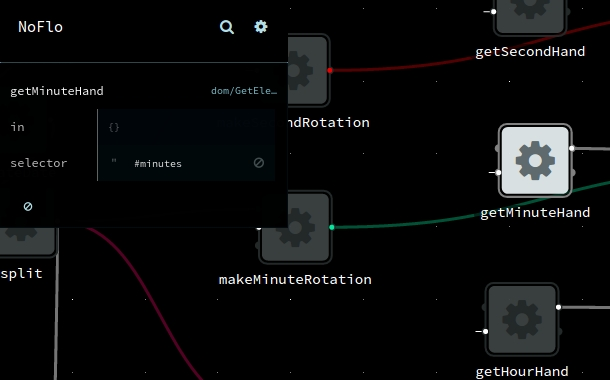
\includegraphics[width=0.86\textwidth]{noflo}
    \caption{Example of node expansion in NoFlo \cite{noflo}}
    \label{fig:noflo}
  \end{center}
\end{figure}

\begin{figure}[t]
  \begin{center}
    \leavevmode
    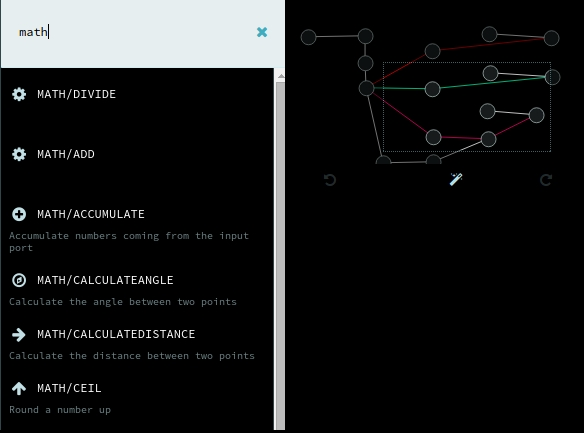
\includegraphics[width=0.86\textwidth]{noflo2}
    \caption{NoFlo node search and minimap navigator \cite{noflo}}
    \label{fig:noflo2}
  \end{center}
\end{figure}

From experimenting with the tool, we found some characteristics that serve as a
lesson of what works well and what doesn't:

\begin{itemize}
  \item A node has the least information possible, yet it can be clicked to
show details, such as some usage notes or seeing some inputs or parameters.
An example of a common NoFlo layout with a node expanded can be seen in Figure
\ref{fig:noflo}. This contributes to saving space in the layout while maintaining
flexibility.
  \item You can search for a block by its name (see Figure \ref{fig:noflo2}).
  \item There is a minimap that helps to navigate the screen, so we can have
a higher level view of the layout \ref{fig:noflo2}).
  \item Weak typing makes it confuse to use some of the nodes, it is unclear
when we can connect input and outputs with mismatching labels, because sometimes
they are compatible and other times they aren't.
  \item Sometimes errors appear immediately, others we can just see them in
runtime. This would be fine as long as it was clear that there was an error,
but that is not the case because the messages blend in with the UI and are
not easily noticeable.
  \item When choosing new blocks, it is often hard to understand what is their
functionality because most nodes have no description other than their name.
  \item Blocks have icons, which presumably provide some visual information
about their functionality (see Figure \ref{fig:noflo2}), but is hard to
understand what the difference between the various icons is. What seems to be a
good idea, to have icons in blocks to identify them by functionality, as the
opposite effect and negatively affects usability.
\end{itemize}

The last four items can convince the reader of the following conclusion: in VPLs, explicit
is better than implicit. Clarity can undoubtedly make all the
difference between a language that can be intuitively used and one that, despite
all its virtues, could take some more time to master.

\subsubsection{RapidMiner}

According to the popular data mining portal KDnuggets' latest tool popularity
poll \cite{kdn}, RapidMiner is the most popular visual tool to use in applied
machine learning. It is also the most complete, featuring 1500 different blocks \cite{rapidminer}.

The product has too many features to be able to deeply analyze each one of them,
including cloud and repository capabilities for storing and sharing work,
mechanisms for deploying models developed locally to a production server or
an API for developing new blocks. RapidMiner is actually more of a suite rather
than just a tool, so in our analysis we'll restrict ourselves to the design of
a model.

The most differentiating factor between RapidMiner and the other VPLs we studied
is that it splits its view between process and results. In the first one, the
user can design the model and then he must run it and go to results to see the output.
Even if goes against the principle of providing immediate feedback to the user
advocated by some VPLs' designers (as discussed in \ref{sec:vp}), it does seem to make
sense in its use case. The reason for that is that production machine learning applications
running batch jobs can take a reasonable amount of time to run, and the analysis
of its results before changing the model can also take some time. This is
different from people using 3D editors (like Blender), where they the trial and
error cycle is much shorter, and users need to get feedback about their changes
much more often.

Having no need to be continuously looking at the output reduces the importance
of it being shown in the same space as the program we're designing, and we can
save space in the layout by moving it to a different tab. On the other hand,
RapidMiner is flexible enough that allows the user to place both the process
and the results windows side by side, so it really is up to the user to decide
how important is it to be seeing everything at the same time. A tool which doesn't
support moving windows and tabs must make a choice whether or not to have the
output shown alongside with the program.

Other strengths of RapidMiner include having error indicators in each block
and thorough descriptions of each
node's functionality, input, output and parameters, including examples. It also
provides visual clues about a node's functionality by using not only meaningful
icons but also colors. This can be observed in Figure \ref{fig:rapidminer},
where file reading nodes are gray, model-related ones green and those related
with data preparation are in pink.

\begin{figure}[t]
  \begin{center}
    \leavevmode
    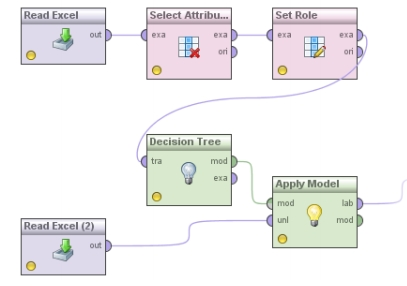
\includegraphics[width=0.86\textwidth]{rapidminer}
    \caption{Classifier in Rapidminer \cite{rapidminer}}
    \label{fig:rapidminer}
  \end{center}
\end{figure}

Something that doesn't seem to work particularly well for someone using the tool
for the first time are the abbreviated labels in the ports. They are cryptic
enough that an inexperienced user has to click the node and read the description
to understand what they are. Maybe it would make sense to either write the full
label for the sake of clarity, or just don't show anything at all.

\subsubsection{Weka Knowledge Flow}

Weka Knowledge Flow is one of the available frontends (others being APIs and a GUI Explorer)
to WEKA's core algorithms \cite{weka}.

\begin{figure}[t]
  \begin{center}
    \leavevmode
    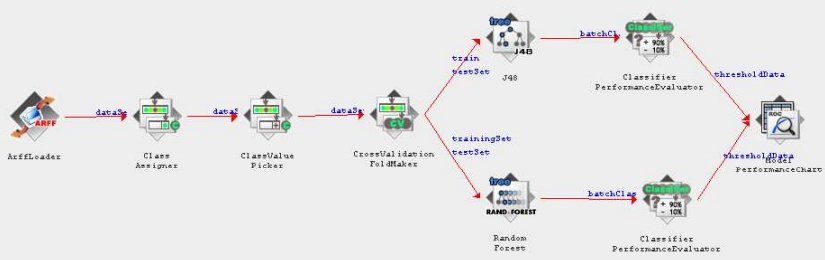
\includegraphics[width=0.86\textwidth]{weka}
    \caption{ROC curve in Weka Knowledge Flow \cite{weka}}
    \label{fig:weka}
  \end{center}
\end{figure}

In this tool, inputs are not connected to specific ports, but rather to a block.
The semantics of the connection is expressed on the edge's label. This can save
some space in the layout as the nodes can be smaller, but in order to understand
a node's input, the user has to waste time following all the edges backward
until he finds the label, which doesn't seem a reasonable tradeoff.

Weka Knowledge makes a good use of icons to differentiate between different node
types. Not only is it easy to the user to distinguish between source, processing
and sink nodes, but also between the different processing nodes' categories
(such as filters, classifiers and clusterers).

\subsubsection{Blender Composite Nodes}

Blender Composite Nodes is part of the Blender open-source 3D computer graphics
software and provides a way for the user to visually build (through a dataflow
representation) a script that can be applied to images or Blender scenes \cite{blender}.

It incorporates common VDP idioms such as source nodes (such as render layers or
RGB), processing nodes (where you can apply blur, shift an RGB curve, etc) and
sink nodes (it's the way to finalize a script and save, or display, the result).
It is interesting to note that
Blender Composite Nodes does not incorporate processing nodes with filter semantics
\footnote{We mean by filter that the result is a subset of the input. Blender has
graphical filters, which are analogous to a functional map operation.},
which is an example of a VPL that intentionally did not incorporate a common
idiom in VDP because it does not make sense for its domain.

\begin{figure}[t]
  \begin{center}
    \leavevmode
    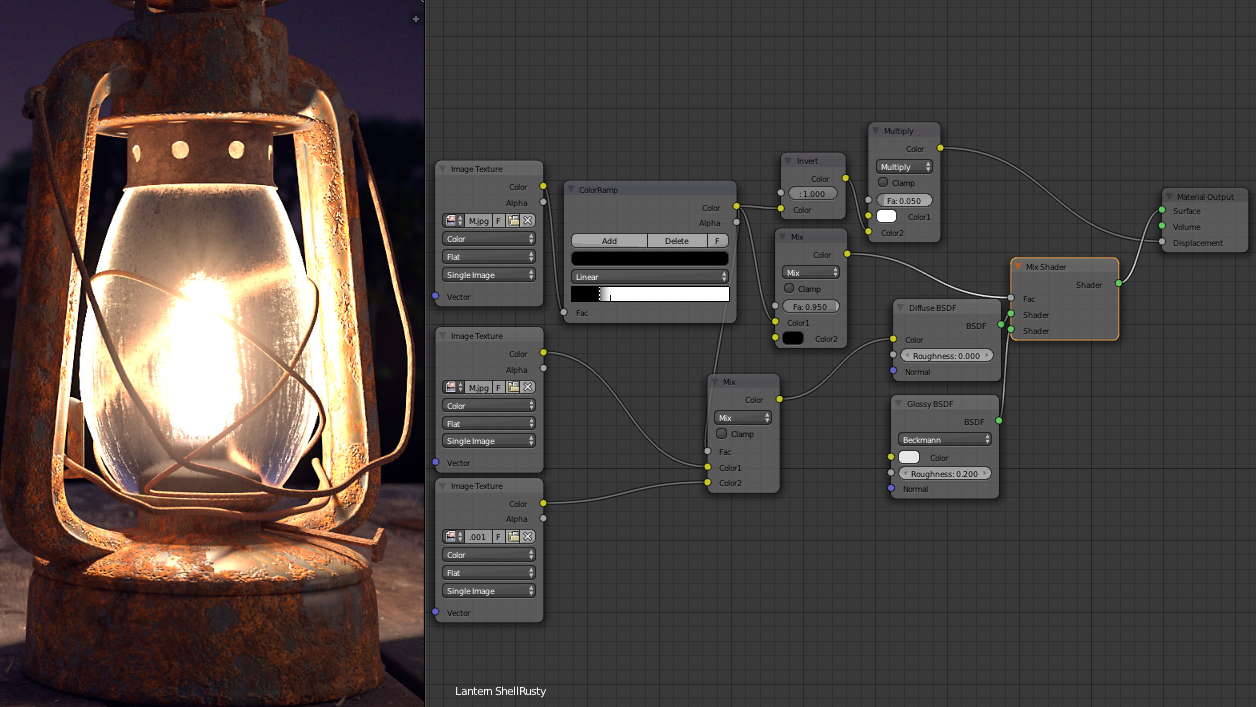
\includegraphics[width=0.86\textwidth]{blender}
    \caption{Script for texture transformation in Blender \cite{blender}}
    \label{fig:blender}
  \end{center}
\end{figure}

There are several interesting characteristics that are worth highlighting:
\begin{itemize}
  \item Composite Nodes assigns a color to each type, so that the user can
easily understand the type of each input or output (see Fig. \ref{fig:blender}).
  \item Implicit conversions for some of the types. For instances,
a conversion from a vector (which are always three-dimensional) to a value yields
the mean of the vector's elements. In figure \ref{fig:blender} we can see that
some values are connected to a different type (among others, the first input
node's color is connected to a simple value named 'Fac'), which is valid behavior.
  \item Incorporating a custom interface within each node. This helps to reduce
the space occupied by the program, since there is no need to create inputs for
every single input in a processing node. It also simplifies the VPL's usage,
because since some types can only exist within certain nodes, and by not being
able to instantiate them outside those nodes, we reduce the possible choices
for input nodes. An example would be the image type enumeration, that we can
see in figure's \ref{fig:blender} input nodes.
  \item Node groups which are essentially an encapsulation
of a set of nodes, resulting in another node that can be re-used, help the user
create his own set of abstractions. Our texture transformation example could
be saved into a node group, so that we can use it in another script without
needing to copy everything from one place to the other or cluttering the new
script's interface with several new nodes. The concept is analogous to functions
in programming.
\end{itemize}

\subsection{VPEs}

In this section we'll be describing three visual programming environments. By VPEs
we mean tools where the user can express the program in a graphical manner that will
later be translated into valid code, regardless of it being executable directly
on the VPE or not.

\subsubsection{Blockly}

Blockly is more than a VPE, it actually is a library for building VPEs \cite{blockly}.
It is fully open source, runs on the browser (in a fully client-side manner) and
was developed to be extensible.

Blockly does not adopt the VDP paradigm, it instead uses a system of blocks
similar to a puzzle, as you can see in Figure \ref{fig:blockly}.
Another useful feature is basic type checking,
so that users can't connect blocks that wouldn't make sense, such as applying an
uppercase function to a number. The way Blockly is built, it is possible to stop the user
from producing an invalid program.

\begin{figure}[t]
  \begin{center}
    \leavevmode
    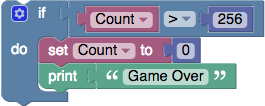
\includegraphics[width=0.86\textwidth]{blockly}
    \caption{Blockly example \cite{blockly}}
    \label{fig:blockly}
  \end{center}
\end{figure}

According to its authors, the reason why they didn't choose to adopt VDP is that
they believe the generated code doesn't look like the VDP graph, making it harder
from a user who later transitions from the tool to textual programming to adapt
to the new format.

It is possible to define new blocks as well completely controlling
how generated code will look like, as well as defining new types. These features
seem to be enough that Blockly can be considered a framework complete enough to
be suitable for building most VPEs and, because it is open-source, it can be
unlimitedly extended.

\subsubsection{Viskell}
\label{sec:viskell}

Viskell is \textit{"an experimental visual programming environment for a typed
(Haskell-like) functional programming language"} \cite{viskell}. Its authors
assume their main goals are, among others, to create a readable and compact
visualizations for functional programming and addressing the scalability issues
of larger visual programs. They state that, in order to achieve the latter goal
and being able to scale up, Viskell should combine a simple core language with
a good type system.

This VPL does not resemble the most popular ones, having some main differences:
the program is designed from top to bottom rather than left to right, blocks
don't have icons but explicit names and all ports have explicit types. This class
of design choices don't seem to be clearly superior to other state of the art tools,
so probably we won't be including them in our VPE.

\begin{figure}[t]
  \begin{center}
    \leavevmode
    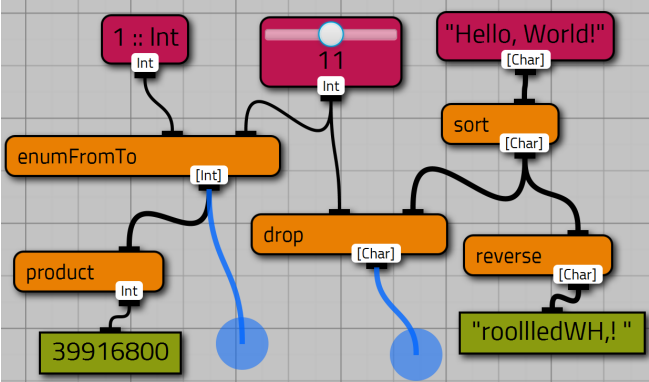
\includegraphics[width=0.86\textwidth]{viskell}
    \caption{Viskell example \cite{viskell}}
    \label{fig:viskell}
  \end{center}
\end{figure}

Nevertheless, there are other interesting features in Viskell, many of which
are tightly coupled to functional programming (such as how it supports currying,
anonymous functions or case expressions). The exception is the capability to
have an incomplete graph and allowing the user to textually insert code to fill
in the gaps (see the blue areas in Figure \ref{fig:viskell}).

Being a work in progress, its authors have pointed out ideas of how to deal with
increased program complexity that they have still not implemented in the language.
Some of them are shown in Figure \ref{fig:viskell2} and outlined below:

\begin{itemize}
  \item Vertical composition of blocks: in the example it is extensively used
in the last ("concatMap") block.
  \item Inline display of constants: as seen in the first block "enumFrom",
where 1 is written inline rather than being a separate source block. It is a form
of horizontal composition.
  \item Functions as constants to higher order functions: represented by the
right-hand side of the 3 blocks in the middle ("map", "groupOn" and "concatMap").
\end{itemize}

This way, we eliminated most of the connections between nodes and achieved a
more compact (we have 4 arcs in a representation that would use more than 20 in
its original format) and readable representation.

\begin{figure}[t]
  \begin{center}
    \leavevmode
    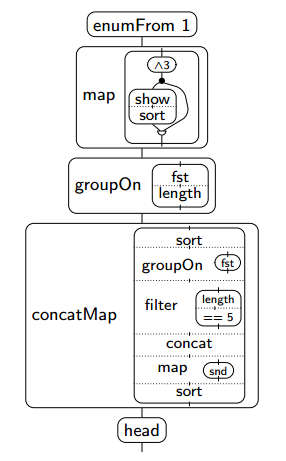
\includegraphics[width=0.86\textwidth]{viskell2}
    \caption{Compressed visual representation example \cite{viskell}}
    \label{fig:viskell2}
  \end{center}
\end{figure}

\subsubsection{WindowBuilder}
\label{sec:winb}

One domain where VPLs have been successfully applied is UI design. Instead of
going through the tedious task of writing boilerplate code (often having to
memorize complicated function signatures) and needing to memorize APIs, users
can just drag and drop elements on the screen.

The Eclipse IDE provides several plugins on its marketplace, one of which is the
WindowBuiler plugin \cite{winbuild} to build Java SWT/Swing UIs.

WindowBuilder is a bi-directional and WISIWIG tool (What You See Is What You Get), meaning
that it generates code that faithfully represents the drawn UI and it is also possible to
directly edit the code and see the updated result back in the design view.

Since defining UIs is a very different domain from PP there are not many features
that we can use from WindowBuilder in our future VPE. The exception is the
bi-directionality of code, which could be useful in certain scenarios.

\begin{figure}[t]
  \begin{center}
    \leavevmode
    \includegraphics[width=0.86\textwidth]{winbuild}
    \caption{WindowBuilder's design view \cite{winbuild}}
    \label{fig:winbuild}
  \end{center}
\end{figure}

\subsection{VIBES}
\label{sec:vibes}

VIBES is a tool, developed by John Winn during his PhD, that allows variational
inference to be performed automatically on a Bayesian network \cite{Winn2005}
defined graphically.
It was written to serve as proof of concept for the variational message passing (VMP)
algorithm, so it has reduced focus on human-computer interaction. Other than its representation
of deterministic inputs with a different edge style than undeterministic ones and
usage of plates to represent loops, from a usability point of view it's not very interesting.

\begin{figure}[t]
  \begin{center}
    \leavevmode
    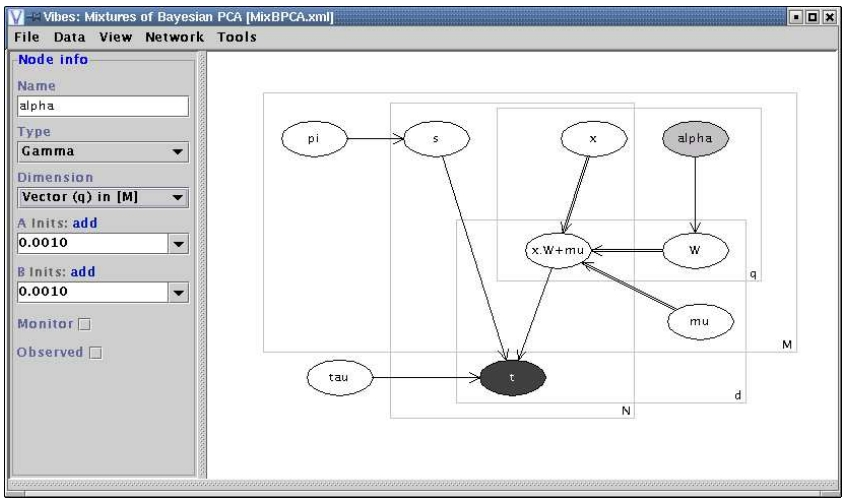
\includegraphics[width=0.86\textwidth]{vibes}
    \caption{Example of a model using VIBES \cite{Winn2005}}
    \label{fig:vibes}
  \end{center}
\end{figure}

\subsection{WinBUGS}
\label{sec:wbugs}

Similarly to VIBES (described in \ref{sec:vibes}), WinBUGS is a framework with a graphical
component which s part of the Bayesian inference Using Gibbs Sampling (BUGS) project.
It allows the user to, graphically or textually, define a model and automatically perform inference
on it (unlike VIBES, the inference algorithm is Gibbs sampling, a method that
resorts to a Markov chain Monte Carlo technique) \cite{Lunn2000}.
Its interface is very similar to VIBES and the only difference between them,
besides the algorithm used, is that WinBUGS provides a bi-directional conversion
between graphical and textual representations.

\begin{figure}[t]
  \begin{center}
    \leavevmode
    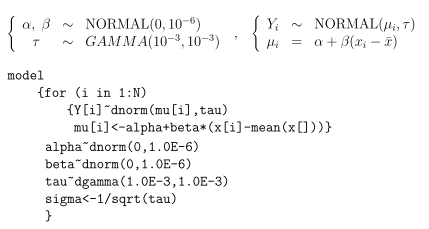
\includegraphics[width=0.86\textwidth]{winbugs}
    \caption{Example of a model translated to WinBUGS textual form \cite{winbugs}}
    \label{fig:winbugs}
  \end{center}
\end{figure}

In Figure \ref{fig:winbugs}, we can see that WinBUG's textual representation of
a simple model can already be harder to understand than the mathematical
formalism it represents. This is exactly the problem we want think it can be
solved with a proper VPE.

\section{Conclusions}

In this section we have seen the application of VP concepts to tools, confirming
the usefulness of many of the concepts studied in the Secton \ref{sec:vp}.

By comparing the different VP applications, we have identified useful features
such as the use of color and icons to transmit meaning, block compression (either
hiding block details or even the grouping of several blocks in different manners),
zooming in and out, minimap navigation, explicit errors, bi-directionality (
being able not only to convert graphics to code, but also vice-versa) and strong typing.

Equally useful to knowing what features are useful is to understand which pitfalls
to avoid, such as not including labels or icons for the sake of having a simpler
interface, resulting being an interface where semantics are too implicit and
hard to capture quickly. One of main goals is to avoid having a VPL that is harder to understand
than the original representation of the model we are developing, similarly to
what happens with WinBUGS textual representation.

\chapter{Solution prototype}\label{chap:chap3}


\section{The problem it solves}

As already described in Section \ref{sec:goals}, this dissertation aims to solve
the problem of PPLs having too much of a steep learning curve for someone who
is unexperienced in programming, even if that person would've enough knowledge
in statistics to leverage PPLs' power in applied machine learning. We propose
to do so by developing a visual programming environment for a PPL that is user-friendly
and yet flexible enough to be able to program solutions for non-trivial problems.

Since the existing work joining VP with PP is still nonexistent, the notable exception
being VIBES and WinBUGS (even if it has its shortcomings, as described in \ref{sec:vibes}),
we have identified margin for improvement.

VPEs have been successfuly
applied to other domains, and considering previous studies in VP that suggest it is
well suited for both limited domains and unexperienced programmers, it is the
author's belief that development in PPLs would also benefit from such a tool.
Therefore, we intend to validate the following hypotehsis:

\begin{quote}
  ``When a user instead of specifying a model textually,
  produces the model via a graphical representation that automatically translates
  itself into executable code, he will do so in a shorter amount of time, make
  fewer errors (both during development and regarding the final solution) and
  will reach a final representation that is more understandable and thus
  easier to maintain.''
\end{quote}

Because there isn't a standard method for evaluating if a language is easier
to work with than another, the question arises on how to evaluate success.
The optimal way to do so would be to make an empiral
study. However, this requires having a tool mature and stable enough so that the
study's results can be considered reliable and representative of an underlying
idea (in this case, that a VPE can boost user's performance when developing
models with a PPL). The goal of this dissertation is to
assess several ways how such a tool could be built, pick one of them and develop
a prototype; is is not to develop production-grade software.

An alternative to this empirical evaluation is to gather examples of probabilistic programs expressed in a
PPL (either the one who chose to serve as backend, or another with similar
capabilities) in its traditional textual form, translate them into our graphical
language, and compare the two forms. This what we will be doing.

\subsection{An empirical study}

The way the study would work would be by compare how fast an user can define a model for a given set of problems
when using a VPL in a regualr way or through our graphical interface. We'd then
count the number of syntax and type erros done with each representation. By
selecting users who never used the given PPL, we could not only measure execution
speed but learning time.

It would also be valuable to assess, not only how fast can someone develop with either
of the alternatives, but also the quality of the output. That could be done in two
steps: starting by verifying if the program correctly models the problem and then
asking the participants in the study if they believe the model they
have developed graphically is easier to understand than its textual counterpart (and
vice-versa).
Although subjetive, we believe getting the participants' opinion
regarding the output quality could provide valuable insights in order to understand if VP can
really enhance an user's experience when using a PPL. Another method we could use
to help us make an assessment of the validity of the hypothesis would be asking
participants questions regarding usability. Even if it may seem redundant, since
we would already have the time measurements, it is a way of identifying strenghts and
weaknesses with reduced granularity.

\subsection{Target audience}

The resulting tool is aimed at people with knowledge in statistics
who are unexperienced programmers. This may include data scientists, researchers,
mathematicians or staticians. In short, anyone who would apply PP to problem
solving but are not fluent in programming.

\subsection{Expected contributions}

By the end of this work, we would expect to have built a VPE for PPLs that can
be extended with more PPLs, even if we are only implementing the adapter for one.
By doing so we will: have a platform that enables other people to experiment
and make usability research on, define a visual language that can be applied to PP in general,
identifying what works and what to avoid,
and ultimately assessing the viability of applying VP to PP to enhance end-user's
productivity.

\section{Outline}

As we have seen in Chapters \ref{chap:intro} and \ref{chap:sota}, there is a
rising awareness of the power of ML methods. PPLs, despite still being mostly
unknown to data scientists, provide an interface for defining personalized
probabilistic models and possess a built-in inference engine.
The benefits of VPLs when compared to a textual format are well-known, but there
is no VPL applied to a PPL, so we aim to create one.

A big requirement we wished to fulfill was, not only ease of use, but also ease
of installation. This means having portability across operating systems as well
as being able to execute without installing dependencies. For this reason, we
decided our VPE should run in the browser.

It was also important that we chose
a target PPL for which there is a decent amount of programs written on it, so we
could thoroughly test our hypothesis. Because it was the one
that best matched this criteria we chose Infer.NET to work with, a framework that
can be used in CLI languages (such as C#, F# or C++). Because none of these
languages can, at least at the time of writing (that might change when WebAssembly
\cite{weba} gets widespread support), be directly compiled to JavaScript
we will be sacrificing immediate
visual feedback and build a hybrid text and visual system (a VPE) rather than a purely
visual language (see Section \ref{sec:vpe} for more details). This means that
our tool won't be able to run the model the user defines, but will generate
Infer.NET (hosted in C#) code (see Figure \ref{fig:scope}).

The user can take the generated
code and run it in a separate runtime (such as CLR). While not the ideal scenario, because it
complicates the development and debugging cycles (in order to see each change,
users must first copy the code to a file in a machine that can compile and run it),
it has the advantage of seamlessly integrating with larger projects. An example
would be an enterprise application written in C# that has a small component
that the team who's developing it feels it would make sense to use a PPL there.
They can use our VPE to develop that portion of the program, and then just place
the code in the desired place. Using a purely visual programming language in the
same scenario, despite having a faster development time, would then require
a rewriting in a textual form.

\begin{figure}[t]
  \begin{center}
    \leavevmode
    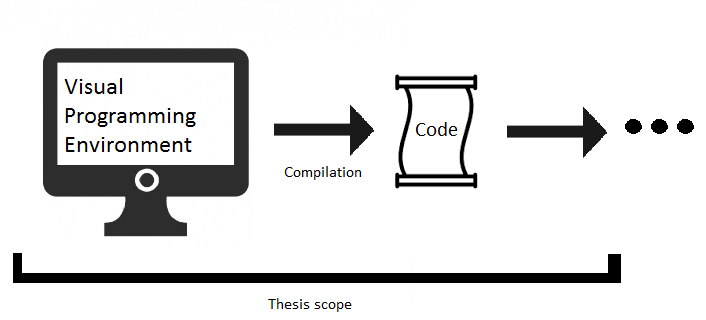
\includegraphics[width=0.86\textwidth]{scope}
    \caption{High-level look into our tool}}
    \label{fig:scope}
  \end{center}
\end{figure}

\section{Architecture}

\section{Implementation}

 % "controlled dataflow vpl"
 In this section we will be explaining why we made certain choices, such as for
 the target PPL, the front-end framework or what features to include or not.

\subsection{Picking a target PPL}
\label{sec:tarppl}

Perhaps one of the most important decisions we had to made concerns the PPL we
would be offering a VPE to, since the visual programming concepts applied are
highly dependent on the language's own capabilities. For instances, we cannot
study how VP can be helpful in an object-oriented design if we are using a
purely functional PPL such as Church which does no have that concept.

As we seen on Section \ref{sec:ppls}, the PPL landscape is heterogeneous enough
that we could pick a language from any paradigm or runtime we wanted to, as there
are many alternatives available. So we could narrow down the scope, we decided to avoid
purely functional and logical programming languages, because we wanted to build
a VPE that was not an end in itself: meaning that it was not only useful to build
PP but also to help our target audience eventually transition from a graphical
environment to the textual form (or, at least, be able to use both if they need
a more fine-grained control in a certain scenario). Even if it is a matter of
debate which paradigm is more suitable to people learning how to program, we feel
that because imperative and object-oriented are more common in data science (the prime
examples being Python and R), they would be a better choice.

After applying this restriction, there were still many PPLs to chose from, so
we decided upon the main criteria on which to make our decision: the language
should have comprehensible and extensive documentation, plenty of code examples
with a variety of complexities, an active and helpful community, be hosted in
a mainstream programming language (as opposed to being a standalone language by itself)
and it should run on the browser. The first three points are related to how well
can we learn the language well enough to design a VPE for it, having no prior
experience with it, in a short amount of time. Being executable on the browser
would allow to provide instant visual feedback of the results, since the VPE
would not be limited to defining a model, but it would could execute it.

On a technical side the strongest candidate is VentureScript \cite{probcomp},
due to the fact it is hosted in javascript (with the aforementioned advantages).
Despite this advantage, it is still on Alpha and both the code examples and
documentation are still scarce, even taking into consideration its predecessor's
examples \cite{forestdb} and tutorials \cite{church}.

The three stronger candidates, after some selection, were PyMC \cite{pymc},
Figaro \cite{figaro} and Infer.NET \cite{InferNET14}. All three are hosted in popular languages
(Python, Scala and C#/F#, respectively) and have comprehensive tutorials and
documentation available \cite{pymct}\cite{figarot}\cite{InferNET14t}.

We ended up choosing Infer.NET because it had the widest range of examples
available, which is pivotal to design a VPE as complete as possible, as well
as evaluate it under different scenarios. Besides its complete documentation
and tutorial, its website features more than 20 code examples, as well as a list
of papers that resorted to Infer.NET. Some of these papers are about PP or PPL theory,
but others are about applications of it, such as "Automatic analysis and
identification of verbal aggression and abusive behaviors for online social
games" \cite{balci2015automatic}, which gives us confidence that Infer.NET is
mature enough so we can focus in the VPE design rather than struggling with
learning the language. Bottom line, it was chosen due to the abundant number of
programs written on it publicly available.

\subsection{Picking a front-end}

After knowing which would be the language we would be targeting, there was still
the need to define both the visual paradigm and the framework, if any, that we
would use to develop the front-end (visual interface) of our VPE.

Regarding the paradigms the two competing alternatives are VDP and the one offered
by Blockly. While the first approach is what we typically see in similar tools,
such as RapidMiner or NoFlo, the second one is a fairly new approach, unseen
in tools other than those which were built using Blockly. It is not trivial to
assess the suitability of either of the options because there was never a study
directly comparing the merits of each of them, so we will try to make our own
analysis by comparing their strenghts and weaknesses while assessing what is
more valuable in the context of a VPE for a PPL.

\subsubsection{Blockly}
\label{sec:fblock}

Similarly to what happens with VP and VPEs, there are plenty of references
in the literature that Blockly-based tools boost productivity \cite{Marron2012} and ease the process
of learning how to program \cite{Junior2006}.

When compared with tools that are
based in a VDP approach, it has a representation that is more similar to how code
is written \cite{blockly}, which can be an advantage in a tool that aims to serve as a visual
interface that generates code in a textual format, such as the one we're developing.
This can be seen as an advantage because, not only does it facilitate fully transitioning
to a textual format as soon as the user is comfortable enough at programming,
but it is also makes it easier to textually fine-tune a code that was developed
using the VPE.

Among the features we analyzed in Section \ref{sec:sotavdp} that deal with
helping the user achieving program correction we saw syntax checking and type
checking. Blockly addresses both situations by visually modeling the program
as a puzzle where only compatible pieces fit together; this is an intuitive way
to enforce correctness, since it maps to an activity the majority of people are
familiarized with: assembling puzzles. This seems a better way to cope with errors
rather than showing an error message at compile or run-time, because often it is
not even clear that there is an error, as we have seen that happens with NoFlo in
Section \ref{sec:noflo}.

Another great advantage of Blockly is that, because it runs on the browser, it is
compatible across devices and operating while not requiring any kind of setup.
If the user choses to download Blockly, it can even work with it without internet
connection. The same applies to our VPE if we chose to build it on top of Blockly.

However, this VPE of VPEs lacks features that enable it to effectively scale up
such as the ones we have seen with NoFlo or Blender Composite Nodes (Section \ref{sec:sotavdp}).
Examples of this include being able to zoom in and out in the UI, searching for
blocks by their name, zoom in and out or create group blocks to encapsulate a certain group of
nodes (a concept analogous to functions in regular programming). It enables the
creation of vertically and horizontally compressed blocks, similarly to Viskell,
by using block composition and dropdowns rather than requiring to plug-in extra blocks
(see Figure \ref{fig:blocklycomp} for an example of each case).

\begin{figure}[t]
  \begin{center}
    \leavevmode
    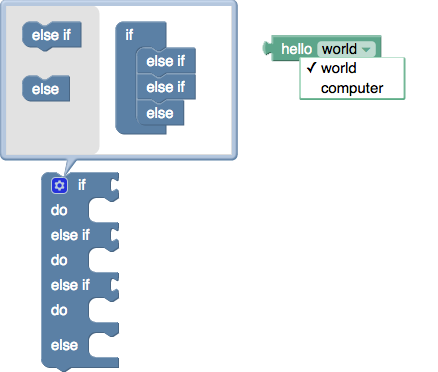
\includegraphics[width=0.86\textwidth]{blocklycomp}
    \caption{Blockly example of horizontal and vertical compression \cite{blockly}}
    \label{fig:blocklycomp}
  \end{center}
\end{figure}

\subsubsection{Eclipse Toolset}

The Eclipse Foundation has some tools, which are accessible as plugins for the
Eclipse IDE, that we thought that could serve as a foundation for the VPE we're
aiming to develop.

Damos \cite{damos}, a project still in the "Proposal" phase of the Eclipse
Development Process, is a framework for building data-flow graphical languages
and their respective code generator. It includes both graphical and textual editors,
as well as support for continuous, synchronous and asynchronous computations.
Even if it already includes enough blocks so it can be used by engineers and scientists
as a replacement for tools like MATLAB/Simulink or LabVIEW, it was designed to
be customizable and extensible with new blocks, so we could use it to build our VPE on.

Damos uses another Eclipse tool as its graphical editor: the Graphical Modeling
Framework (GMF). GMF can be used to build graphical editors for multiple visual
languages \cite{gmf}, such as UML modeling, application interfaces such as the
one described in Section \ref{sec:winb} or, eventually, a visual language for a
PPL. GMF is often used in conjunction with the Eclipse Modeling Framework (EMF),
"a modeling framework and code generation facility for building tools and other
applications based on a structured data model" \cite{emf}.

In spite of their advantages, all of these have two common problems. First, they require
users to download both Eclipse and the used plugins and their dependencies
which not only constitutes an entry barrier but hinders collaboration, because
it makes it difficult to share the model among colleagues. And secondly, they
were built to generate code to specific target languages (C for Damos and Java
for EMF), neither of which has a PPL implementation with a strong community
(Probabilistic-C \cite{Paige2014} serves as a proof of concept and we already explained
in Section \ref{sec:tarppl} why we discarded Figaro). Even if we could eventually
use the generated C or Java as an intermediary representation, we believe the
extra burden (both in development time and in runtime performance) of having an
extra transformation does not justify for the added benefits when compared with
other front-ends.

\subsubsection{Custom implementation}

At this point the strongest candidate for a front-end was Blockly,
but it would also be possible to fully develop a new front-end, instead of using
a framework such as Blockly or the tools from the Eclipse toolset. The purpose of
doing so would be overcoming Blockly's limitations that we refered earlier in
Section \ref{sec:fblock}. In order to keep Blockly's portability, we would have an
implementation targeting the browser, where the visual elements would be
represented by DOM tree elements and drawn using the browser's render engine,
just like a regular HTML page; for performance reasons, we could use the HTML
\textit{canvas} element \cite{w3ccanvas}.

The reason why we won't be choosing this option is that we believe that this
flexibility of implementing extra features, that essentially have to do with
navigation and block filtering or selection, are not worth the risk of having
a VPE that does not feel as fluid and as natural as Blockly or GMF implementation would, since all
those aforementioned features are secondary when compared to the look and feel
of the core VPE (by core we mean the workspace where we drag the blocks, edit
their inline properties and connect them).

Examples of such core usability features, besides having a layout that has already been
tested (proven to deliver the benefits of VP)
that Blockly already provides include magnetic connections
(you don't have to drag and drop a block to a stricly defined area, doing so near
a valid connection highlights that connection and makes it possible to drop it there)
and block mutations (a block may change when you connect certain blocks to it,
this allows for horizontal and vertical compression).

Using a third-party framework also has the advantage of automatically getting new
features as soon as that framework is updated, such as the zoom in and out that
Blockly is planning to deliver \cite{blockly}.

\section{Development steps}

The purpose of this section is to enumerate the difficulties encountered when
developing a VPE that could support the design of programs similar in functionality
to the ones the reader can find in Infer.NET's tutorials \cite{InferNET14t} and
the solution we adopted to overcome them.

\subsection{Generating basic C#}

Since Infer.NET is hosted in C# but Blockly does not include a generator for
the language, the first thing to do was to be able to provide code generation for
Blockly's default blocks, that provide a language's most basic constructs such
as variables, lists and control structures.

We decided to adopt an open-source implementation to solve this issue \cite{csgen}
but since it was not compatible with Blockly's versions since January 2016, it
was necessary to work on making it compatible, so we could have the latest features
available, such as zooming in and out, which we had previously identified as a
major feature required in a VPE to be able to scale up programs visually.

This work lead to the pull request \#8 to that open-source project \cite{csgenpr}.

\subsection{Mandatory declarations}

Similarly to Java and C/C++, in order to run a program, you must provide a method
as an entry point, where the control flow will start and end. However, a textual
representation generated by Blockly does not comtemplate this possibility, so
we had to figure out how to deal with this issue. Figure \ref{fig:before} shows a simple program,
and this is its generated code:

\begin{figure}[t]
  \begin{center}
    \leavevmode
    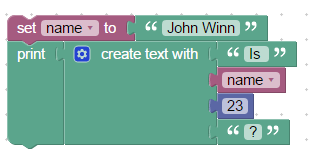
\includegraphics[width=0.86\textwidth]{before}
    \caption{Blockly simple example}
    \label{fig:before}
  \end{center}
\end{figure}

\begin{lstlisting}
dynamic name;


name = "John Winn";
Console.WriteLine(String.Concat("Is ", name, 23, "?"));
\end{lstlisting}

If you try to run this code you will get a compile-time error, as expected.

Another issue that arises when representing Infer.NET programs in Blockly is how
to specify inference engine settings, such as the algorithm is should use, if it
parallelizes for-loops, if it re-allocates internal messages between inference
runs, etc. Unlike other kinds of statements, such as loops, variable declarations
or prints, these settings are usually only set once per program and remain
unaltered.

Having both these situations in mind, a possible solution is to use a singleton
block (one that must be present in every representation and can't be deleted),
where we aggregate both these concerns and which contains the remainder of the program.
Such an example can be seen in Figure \ref{fig:after}, which generates the following code:

\begin{figure}[t]
  \begin{center}
    \leavevmode
    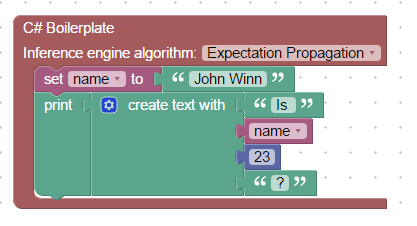
\includegraphics[width=0.86\textwidth]{after}
    \caption{Blockly simple example with C# boilerplate}
    \label{fig:after}
  \end{center}
\end{figure}

\begin{lstlisting}
using System;
using System.Collections.Generic;
using System.Text;
using MicrosoftResearch.Infer.Models;
using MicrosoftResearch.Infer;

namespace InferBlockly
{
	public class InferBlockly
	{
		public void Run()
		{
			InferenceEngine engine = new InferenceEngine();
			engine.Algorithm = new ExpectationPropagation();
			dynamic name;


			name = "John Winn";
			Console.WriteLine(String.Concat("Is ", name, 23, "?"));
		}
	}
}
\end{lstlisting}

Despite losing flexibility, since it is impossible to change the settings
throughout the program (even if that is valid in Infer.NET),
we believe that this increased simplicity is more intuitive and therefore benefitial to an unexperienced
programmer than allowing the settings to be changed at any point in time.

\subsection{Variable type checking}

Every PPL has the concept of random variables, which are the building block of
any PP. Some examples in Infer.NET are listed below.

\begin{lstlisting}
  			Variable<bool> firstCoin = Variable.Bernoulli(0.5).Named("firstCoin");
        Variable<double> x = Variable.GaussianFromMeanAndVariance(0, 1).Named("x");
        Variable<double> threshold = Variable.New<double>().Named("threshold");
        Variable<double> precision = Variable.GammaFromShapeAndScale(1, 1).Named("precision");
        VariableArray<double> x = Variable.Array<double>(dataRange).Named("x");
        VariableArray<bool> y = Variable.Observed(willBuy).Named("y");
\end{lstlisting}

Because there are so many different types (we are showing 4, but there are more),
we believe our VPE should help the user avoid mistakes related with using wrong
types, such as trying to apply logical operators to numeric random variables or
greater than comparisons between boolean variables.

When choosing how to represent variables we had to take into account that
Blockly was conceived to target dynamic languages, as it can be seen by the languages
it targets: JavaScript, Python, PHP and Dart (which supports static type-checking,
but it's not the default mode \cite{dart}). The negative consequence of this is that it's
not ready to perform type checking on variables, meaning that an user can
produce invalid programs when using variables (as seen in Figure \ref{fig:valid_blockly}, we have
drawn a program that will produce a runtime exception, since we can't evalaute
the square root of a text string), althought the same doesn't happen when
directly connecting the blocks, since we can't connect text input blocks to the
right connector of the square root block.

There have been dicussions among open-source projects that rely on Blockly on how
to incorporate type checking for variables (such as a VPE for Arduino \cite{bduino}
or one for Kiwi.js \cite{gbl}, an HTML5 game framework) as well as in Blockly's
dicussion forum \cite{gbl2}, but none reached a final proposal, let along a working
implementation.

Therefore, we have decided to extend Blockly in order to be able to support
different types of variables with a similar type check to the one used in other
kinds of blocks, meaning that if they don't type check, the pieces don't fit and the user
can't connect them. This was done by adding an extra field to FieldVariable
(the class Blockly class that represents variables) that identifies its type and
modifying the behavior of each component that deals with variables to take that
into account \footnote{These changes can be found in github.com/gcandal/blockly/commit/8f5fa0}.

This way, variables from different types are kept isolated, so that if the user
declares a boolean variable named \textit{bool}, it won't appear in numeric
variable's dropdowns or menus. This segregation between different variable types,
besides allowing to have the aforementioned type checking at the block level, it
also allows to have different colors and labels in the blocks for different types of variables
(making it clearer to the user they should be used differently) and to declare
explicit C# types in the generated code, rather than using
the dynamic keyword to avoid static type-checking \cite{cdyn}. The advantage is that
the generated code is closer to the one that would be written by a programmer,
so it eases the transition from a VPE to a textual format, since both representations
are similar.

\begin{figure}[t]
  \begin{center}
    \leavevmode
    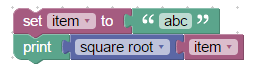
\includegraphics[width=0.86\textwidth]{valid_blockly}
    \caption{Blockly example of representable invalid program}
    \label{fig:valid_blockly}
  \end{center}
\end{figure}

\subsection{Serialization}

It is important in a VPE to be able to save and load programs, so the user can
not only work on a given program at different points in time, but also share it
with other users. Blockly makes it possible to do so by converting a graphical
representation to XML, which can later be imported.

\section{Limitations}

In this section we will describe some limitations that our chosen toolset (using
Blockly to represent Infer.NET C#) imposes in functionality.

\subsection{Inverse compilation}

By inverse compilation we mean the act of converting a program in a textual form
to its Blockly representation. This could be useful because it would help users
easily switch between representations, similarly to Window Builder (as discussed in Section \ref{sec:winb})
and unlike what happens with our current approach.
With our VPE, if you textually make a change in the program,
and since that won't be reflected in the graphical representation, everytime
the code is re-generated (which happens frequently and unexpectedly, in situations
such as opening and closing menu tabs) your changes will be overriden.

Even if parsing C# and converting it to an intermediate representation would be
simple (Microsoft provides an EBNF grammar for the language \cite{ebnfcs}), there
are a number of questions that should be answered before implementing this feature.
For instances, our graphical representation guarantees type safety and a valid
program so it would not make sense to allow specifying an invalid program that
would be translated into a graphical form, it would break one of the most important
guarantess, the one that makes it suitable for beginners in programming. In
order to ensure a valid textual program, we would need to be able to either mimick
the compiler's verifications or run the compiler itself; the first option is
a big challenge while the second is incompatible with the VPE being browser-based
(the compiler does not run, and cannot be easily converted to JavaScript).

\subsection{Instant visual results}

As we discussed before in several parts of this work, a big tradeoff we made was
to sacrifice the flexibility of using any language needed in favor of the portability
of a VPE that runs in the browser, which (as of this moment) only runs JavaScript.

Perhaps the greatest limitation of this approach is not being able to run Infer.NET
code, which makes it impossible not to violate the VP principle of instant visual results.
The development cycle is greatly affected by forcing the user to copy the text
into a location where a compiler can access and run it. A work around for this
would be to adopt a client-server architecture where our server would run the code
and send the results back to the user. Even if that creates a need for internet
connection, which currently does not exist, we believe it to be a worthwhile tradeoff
and something to pursue in future work.

Currently we can only show the generated code in real time, but we took special
care to have an interface where the user can see both representation simultaneously
without having to perform any actions such as switching between tabs or pressing
a \textit{'Generate code'} button, so we could minimize this possible as best as we could
without adopting the client-server architecture.

\subsection{Object-oriented programming}

You may notice that, even while we're targeting an object-oriented programming
language, our VPE has no support for representing classes. It also does not
support file management (splitting the program in several files) or namespaces.

The reason for this is that our target audience is not concerned with those features.
As discussed in Section \ref{sec:vp} VP is best suited for small domains, and our
VPE is meant to help data scientists and statisticians with little or no programming
experience start getting familiar with PP through a PPL, and not provide a
fully featured IDE.

Incorporating this kind of features, although feasible, would significantly
make the VPE more complex both in terms of cluttering the interface and the user
experience by providing mostly unecessary options, thus having little added
benefit to the majority of users.

\section{Tutorial}

\section{Conclusions}

\chapter{Evaluation}\label{chap:chap4}

\section*{}

\section{Problems solved}

\section{Problems detected}

\section{Conclusions}

\chapter{Conclusions} \label{chap:concl}

\section*{}

\section{Future Work}

In the time I'll be dedicated to accomplish what I have proposed to do, developing
a visual programming environment and gathering knowledge of what works best in
a visual representation and what doesn't, I'll be following the work plan presented
in Figure \ref{fig:workplan}.

During these nearly 5 months, the plan is to start weighting the pros and cons
of using certain PPLs and picking one of them to be used. The next step would be
picking an apropriate frontend, deciding between Blockly, a custom HTML+Javascript
solution, or other alternative. Then, I'll start by gathering the fundamental
language constructs that must be included, defining how they could be represented
in the visual language and developing the frontend and code generation for those constructs.
From this point onwards until the end, I've planned to make iterations: of choosing
new language features to integrate, adapt the frontend and code generation for them,
converting textual examples to the visual representation and studying the differences
between the two representations. Finnally, there
will be some time to make a tutorial on how to use the VPE.

\begin{figure}[t]
  \begin{center}
    \leavevmode
    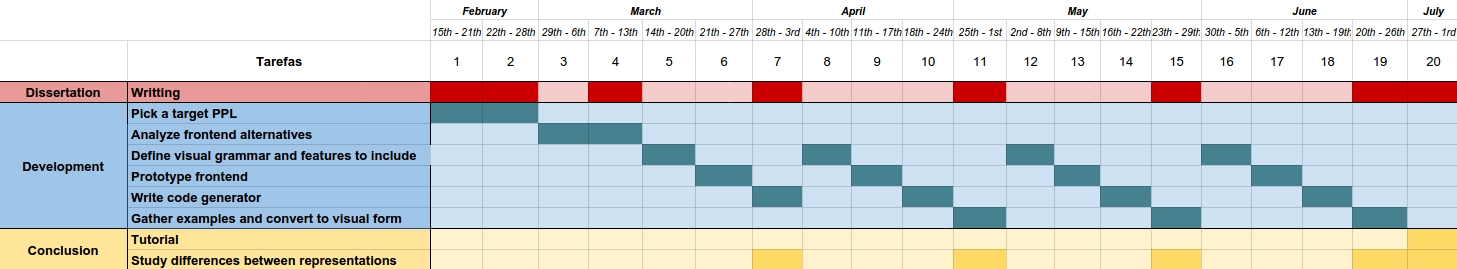
\includegraphics[width=0.86\textwidth]{workplan}
    \caption{Work plan for the work of this dissertation}
    \label{fig:workplan}
  \end{center}
\end{figure}

\chapter{Conclusions} \label{chap:concl}

\section*{}

Critical analysis: when to use or not, strengths and weaknesses.

\section{Limitations}

In this section we will describe some limitations that our chosen toolset (using
Blockly to represent Infer.NET C#) imposes in functionality.

\subsection{Inverse compilation}

By inverse compilation we mean the act of converting a program in a textual form
to its Blockly representation. This could be useful because it would help users
easily switch between representations, similarly to Window Builder (as discussed in Section \ref{sec:winb})
and unlike what happens with our current approach.
With our VPE, if you textually make a change in the program by directly
writing in the text-area where it appears,
and since that won't be reflected in the graphical representation, every time
the code is re-generated (which happens frequently and unexpectedly, in situations
such as opening and closing menu tabs) your changes will be overridden.

Even if parsing C# and converting it to an intermediate representation would be
simple (Microsoft provides an EBNF grammar for the language \cite{ebnfcs}), there
are a number of questions that should be explored before implementing this feature.
For instances, our graphical representation guarantees type safety and a valid
program so it would not make sense to allow specifying an invalid program that
would be translated into a graphical form, it would break one of the most important
guarantees, the one that makes it suitable for beginners in programming. In
order to ensure a valid textual program, we would need to be able to either mimic
the compiler's verifications or run the compiler itself; the first option is
a big challenge while the second still requires further investigation on how
to handle users' errors.

\subsection{Instant visual results}

As we discussed before in several parts of this work, a big tradeoff we made was
to sacrifice the flexibility of using any language needed in favor of the portability
of a VPE that runs in the browser, which (as of this moment) only runs JavaScript.

Perhaps the greatest limitation of this approach is not being able to run Infer.NET
code, which makes it impossible not to violate the VP principle of instant visual results.
The development cycle is greatly affected by forcing the user to copy the text
into a location where a compiler can access and run it. A workaround for this
is to adopt a client-server architecture where our server would run the code
and send the results back to the user. Even if that creates a need for internet
connection, which currently does not exist, we believe it to be a worthwhile tradeoff
and so we have chosen to implement it.

The downside of this approach is that we have to wait for the round-trip time
of the program to be sent to the server plus the compilation and execution times.
During this process, the user does not get any feedback; this could be minimized
by providing push notifications to the client and streaming the program's output,
rather than waiting for the execution to finish to get a response.

\subsection{Object-oriented programming}

You may notice that, even while we're targeting an object-oriented programming
language, our VPE has no support for representing classes. It also does not
support file management (splitting the program in several files) or namespaces.

The reason for this is that our target audience is not concerned with those features.
As discussed in Section \ref{sec:vp} VP is best suited for small domains, and our
VPE is meant to help data scientists and statisticians with little or no programming
experience start getting familiar with PP through a PPL, and not provide a
fully featured IDE.

Incorporating this kind of features, although feasible, would significantly
make the VPE more complex both in terms of cluttering the interface and the user
experience by providing mostly unnecessary options, thus having little added
benefit to the majority of users.

\section{Future Work}

During the work of this thesis, we have certainly identified areas where there
could be improvements. The first one is an addition to the validation process, while the
second concerns a feature that could be added; we describe both below.

Besides these two, the concepts we explore in this text could be further improved,
and even extended, by continuing to perform the example modeling loop.
Even if we feel that we have tackled the most significant
challenges, and provided a decent number of examples, there is always still more
work to be done in this area.

Using examples from a different PPL could be interesting, even if the semantics
are usually very similar, so we could access the generality of the concepts
and transformation patterns we have been studying.

Another feature that would highly value the VP tools for PP in respect to their
textual counterparts would be to include more visual feedback. This includes
not only graphics of the resulting distributions, but could even show progress
while the model is running, so the user could debug their program.

\subsection{An empirical study}

As discussed in Chapter \ref{chap:chap3}, an interesting approach to further validate
the hypothesis that a change in paradigm from traditional procedural or
object-oriented PP to visual PP makes a certain class of users more productive
would be to perform an empirical study whose participants would belong to the
target audience we defined in Section \ref{sec:audience}.

The way the study would work would be by compare how fast a user can define a model for a given set of problems
when using a PPL in a regular way or through our graphical interface. We'd then
count the number of syntax and type errors done with each representation. By
selecting users who never used the chosen PPL, we could not only measure execution
speed but learning time.

It would also be valuable to assess, not only how fast can someone develop with either
of the alternatives, but also the quality of the output. That could be done in two
steps: starting by verifying if the program correctly models the problem and then
asking the participants in the study if they believe the model they
have developed graphically is easier to understand than its textual counterpart (and
vice-versa).
Although subjective, we believe getting the participants' opinion
regarding the output quality could provide valuable insights in order to understand if VP can
really enhance a user's experience when using a PPL. Another method we could use
to help us make an assessment of the validity of the hypothesis would be asking
participants questions regarding usability. Even if it may seem redundant, since
we would already have the time measurements, it is a way of identifying strengths and
weaknesses of the visual representation.

\subsection{Function blocks}

A feature that was left out during development but could have a significant
impact in the VPE's usability, mainly during the development of large models
(scaling up) would be to provide the user with the capability to create his own
blocks, made up of smaller blocks. This is analogous to functions in regular
programming and has been successfully applied to widely used VPE, as we have
seen in \ref{chap:sota}.


%%----------------------------------------
%% Final materials
%%----------------------------------------

%% Bibliography
%% Comment the next command if BibTeX file not used
%% bibliography is in ``myrefs.bib''
\PrintBib{myrefs}

%% comment next 2 commands if numbered appendices are not used
% \appendix
% \chapter{Loren Ipsum} \label{ap1:loren}

Depois das conclusões e antes das referências bibliográficas,
apresenta-se neste anexo numerado o texto usado para preencher a
dissertação.

\section{O que é o \emph{Loren Ipsum}?}

\emph{\textbf{Lorem Ipsum}} is simply dummy text of the printing and
typesetting industry. Lorem Ipsum has been the industry's standard
dummy text ever since the 1500s, when an unknown printer took a galley
of type and scrambled it to make a type specimen book. It has survived
not only five centuries, but also the leap into electronic
typesetting, remaining essentially unchanged. It was popularised in
the 1960s with the release of Letraset sheets containing Lorem Ipsum
passages, and more recently with desktop publishing software like
Aldus PageMaker including versions of Lorem Ipsum~\citep{kn:Lip08}. 

\section{De onde Vem o Loren?}

Contrary to popular belief, Lorem Ipsum is not simply random text. It
has roots in a piece of classical Latin literature from 45 BC, making
it over 2000 years old. Richard McClintock, a Latin professor at
Hampden-Sydney College in Virginia, looked up one of the more obscure
Latin words, consectetur, from a Lorem Ipsum passage, and going
through the cites of the word in classical literature, discovered the
undoubtable source. Lorem Ipsum comes from sections 1.10.32 and
1.10.33 of ``de Finibus Bonorum et Malorum'' (The Extremes of Good and
Evil) by Cicero, written in 45 BC. This book is a treatise on the
theory of ethics, very popular during the Renaissance. The first line
of Lorem Ipsum, ``Lorem ipsum dolor sit amet\ldots'', comes from a line in
section 1.10.32.

The standard chunk of Lorem Ipsum used since the 1500s is reproduced
below for those interested. Sections 1.10.32 and 1.10.33 from ``de
Finibus Bonorum et Malorum'' by Cicero are also reproduced in their
exact original form, accompanied by English versions from the 1914
translation by H. Rackham.

\section{Porque se usa o Loren?}

It is a long established fact that a reader will be distracted by the
readable content of a page when looking at its layout. The point of
using Lorem Ipsum is that it has a more-or-less normal distribution of
letters, as opposed to using ``Content here, content here'', making it
look like readable English. Many desktop publishing packages and web
page editors now use Lorem Ipsum as their default model text, and a
search for ``lorem ipsum'' will uncover many web sites still in their
infancy. Various versions have evolved over the years, sometimes by
accident, sometimes on purpose (injected humour and the like). 

\section{Onde se Podem Encontrar Exemplos?}

There are many variations of passages of Lorem Ipsum available, but
the majority have suffered alteration in some form, by injected
humour, or randomised words which don't look even slightly
believable. If you are going to use a passage of Lorem Ipsum, you need
to be sure there isn't anything embarrassing hidden in the middle of
text. All the Lorem Ipsum generators on the Internet tend to repeat
predefined chunks as necessary, making this the first true generator
on the Internet. It uses a dictionary of over 200 Latin words,
combined with a handful of model sentence structures, to generate
Lorem Ipsum which looks reasonable. The generated Lorem Ipsum is
therefore always free from repetition, injected humour, or
non-characteristic words etc. 


%% Index
%% Uncomment next command if index is required
%% don't forget to run ``makeindex mieic-en'' command
%\PrintIndex

\end{document}
